\documentclass[10pt]{beamer}

\usepackage[T1]{fontenc}

\usetheme{metropolis}

\usepackage{graphicx}
\usepackage{animate}
\graphicspath{{images/}}
\usepackage{amsmath, amssymb, amsthm}
\usepackage{mathtools}
\usepackage{bm}
\usepackage{booktabs}
\usepackage{caption}
\usepackage{array}
\usepackage{tikz}
\usetikzlibrary{positioning, arrows.meta, calc}
\usepackage{listings}
\usepackage{xcolor}
\usepackage[numbers,square]{natbib}
\usepackage[most]{tcolorbox}
\usepackage{tabularx}
\definecolor{codebg}{RGB}{245,245,245}
\definecolor{codeframe}{RGB}{180,180,180}
\definecolor{boxbg}{RGB}{235,245,255}
\definecolor{boxframe}{RGB}{70,130,180}
\definecolor{ctrl}{HTML}{EB6834}   % P.ORANGE: the control, as in the figures

\lstdefinestyle{pytorch}{
  language=Python,
  basicstyle=\ttfamily\scriptsize,
  keywordstyle=\color{blue!70!black}\bfseries,
  stringstyle=\color{green!50!black},
  commentstyle=\color{gray}\itshape,
  showstringspaces=false,
  breaklines=true,
  columns=fullflexible,
  backgroundcolor=\color{codebg},
  frame=single,
  rulecolor=\color{codeframe},
  framesep=4pt,
  xleftmargin=4pt,
  xrightmargin=4pt,
}
\lstset{style=pytorch}

\title{Introduction to Control Theory}
\subtitle{Mathematical Foundations of Control and Machine Learning}
\author{Enrique Zuazua, Daniel L\'opez Montero}
\date{Winter 2026}
\institute{FAU Erlangen-N\"urnberg}

% --- Math shortcuts --------------------------------------------------------
\newcommand{\R}{\mathbb{R}}
\newcommand{\N}{\mathbb{N}}
\newcommand{\Kal}{\mathcal{K}}
\newcommand{\Gram}{\mathcal{G}}
\newcommand{\Reach}{\mathcal{R}}
\newcommand{\Uad}{\mathcal{U}_{\mathrm{ad}}}
\newcommand{\ctrl}[1]{\textcolor{ctrl}{#1}}
\DeclareMathOperator{\Range}{Range}
\DeclareMathOperator{\rank}{rank}

% --- A box for definitions and theorems ------------------------------------
\newtcolorbox{mathbox}[2][]{
  colback=boxbg, colframe=boxframe, boxrule=0.2pt, arc=2pt,
  left=4pt, right=4pt, top=2pt, bottom=2pt,
  title=\textbf{#2}, fonttitle=\small, coltitle=white, colbacktitle=boxframe,
  halign=left, #1}

% --- Notebook references for worked examples and exercises only ------------
\newcommand{\nbref}[1]{%
  \begin{tikzpicture}[remember picture, overlay]
    \node[anchor=south west, font=\scriptsize, text=black!55]
      at ([xshift=5mm, yshift=1.1mm] current page.south west) {Notebook #1};
  \end{tikzpicture}}

\setbeamerfont{standout}{size=\Large, series=\mdseries}
\setbeamertemplate{bibliography item}[text]
\renewcommand{\bibsection}{}

% --- Bibliography database -------------------------------------------------
% The entries live here so that the slides are one self-contained file.  Each
% compilation writes them to introduction_control_theory.bib for BibTeX: edit
% this block, not the generated .bib file.
\begin{filecontents}[overwrite]{introduction_control_theory.bib}
@article{maxwell1868,
  author  = {Maxwell, James Clerk},
  title   = {On Governors},
  journal = {Proceedings of the Royal Society of London},
  volume  = {16},
  pages   = {270--283},
  year    = {1868},
  doi     = {10.1098/rspl.1867.0055}
}

@book{wiener1948,
  author    = {Wiener, Norbert},
  title     = {Cybernetics: or Control and Communication in the Animal and the Machine},
  publisher = {MIT Press},
  address   = {Cambridge, MA},
  year      = {1948}
}

@article{bellman1954,
  author  = {Bellman, Richard},
  title   = {The Theory of Dynamic Programming},
  journal = {Bulletin of the American Mathematical Society},
  volume  = {60},
  pages   = {503--515},
  year    = {1954},
  doi     = {10.1090/S0002-9904-1954-09848-8}
}

@book{pontryagin1962,
  author    = {Pontryagin, Lev S. and Boltyanskii, Vladimir G. and Gamkrelidze, Revaz V. and Mishchenko, Evgenii F.},
  title     = {The Mathematical Theory of Optimal Processes},
  publisher = {Interscience},
  address   = {New York},
  year      = {1962}
}

@article{kalman1960,
  author  = {Kalman, Rudolf E.},
  title   = {Contributions to the Theory of Optimal Control},
  journal = {Bolet\'in de la Sociedad Matem\'atica Mexicana},
  volume  = {5},
  pages   = {102--119},
  year    = {1960}
}

@article{kalman1960filter,
  author  = {Kalman, Rudolf E.},
  title   = {A New Approach to Linear Filtering and Prediction Problems},
  journal = {Journal of Basic Engineering},
  volume  = {82},
  number  = {1},
  pages   = {35--45},
  year    = {1960},
  doi     = {10.1115/1.3662552}
}

@book{sontag1998,
  author    = {Sontag, Eduardo D.},
  title     = {Mathematical Control Theory: Deterministic Finite Dimensional Systems},
  edition   = {2},
  publisher = {Springer},
  address   = {New York},
  year      = {1998},
  doi       = {10.1007/978-1-4612-0577-7}
}

@book{coron2007,
  author    = {Coron, Jean-Michel},
  title     = {Control and Nonlinearity},
  series    = {Mathematical Surveys and Monographs},
  volume    = {136},
  publisher = {American Mathematical Society},
  address   = {Providence, RI},
  year      = {2007},
  doi       = {10.1090/surv/136}
}

@incollection{zuazua2007,
  author    = {Zuazua, Enrique},
  title     = {Controllability and Observability of Partial Differential Equations: Some Results and Open Problems},
  booktitle = {Handbook of Differential Equations: Evolutionary Equations},
  volume    = {3},
  publisher = {North-Holland},
  address   = {Amsterdam},
  pages     = {527--621},
  year      = {2007},
  doi       = {10.1016/S1874-5717(07)80010-7}
}

@book{astrommurray2021,
  author    = {{\AA}str{\"o}m, Karl J. and Murray, Richard M.},
  title     = {Feedback Systems: An Introduction for Scientists and Engineers},
  edition   = {2},
  publisher = {Princeton University Press},
  address   = {Princeton, NJ},
  year      = {2021}
}

@book{nelson1967,
  author    = {Nelson, Edward},
  title     = {Tensor Analysis},
  publisher = {Princeton University Press},
  address   = {Princeton, NJ},
  year      = {1967}
}

@techreport{hoag1969,
  author      = {Hoag, David G.},
  title       = {The History of {Apollo} On-board Guidance, Navigation, and Control},
  institution = {MIT Charles Stark Draper Laboratory},
  number      = {P-357},
  year        = {1976}
}

@article{luenberger1964,
  author  = {Luenberger, David G.},
  title   = {Observing the State of a Linear System},
  journal = {IEEE Transactions on Military Electronics},
  volume  = {8},
  number  = {2},
  pages   = {74--80},
  year    = {1964},
  doi     = {10.1109/TME.1964.4323124}
}
\end{filecontents}

\begin{document}

\maketitle

% =========================================================================
\begin{frame}{Plan of the lecture}
\begin{columns}[T]
\begin{column}{0.5\textwidth}
\alert{\textbf{Part I.}} Dynamical systems, control and the three questions
\begin{enumerate}
\item A short history
\item Dynamical systems
\item Acting on a system: the ingredients of a control problem
\item The linear setting and the harmonic oscillator
\item Optimal control, controllability, feedback;
\end{enumerate}
\end{column}
\begin{column}{0.5\textwidth}
\alert{\textbf{Part II.}} Controllability of linear systems
\begin{enumerate}\setcounter{enumi}{5}
\item The reachable set
\item The Kalman rank condition
\item Combining motions: parking
\item The Gramian and an explicit control; the cost of control
\item Control and learning; outlook
\end{enumerate}
\end{column}
\end{columns}

\bigskip
\small
Notebooks \textbf{01} and \textbf{02} of the course complement these slides with proofs, worked examples, code and exercises.
\end{frame}


\begin{frame}[standout]
Part I

\medskip
\normalsize Dynamical systems, control and the three questions
\end{frame}


% =========================================================================
\section{A short history}

\begin{frame}{Regulators before the theory}
\begin{columns}[T]
\begin{column}{0.48\textwidth}
\footnotesize
\begin{minipage}[t][2.9cm][t]{\linewidth}
\raggedright
\alert{Third century BCE.} Ktesibios' water clock keeps its water supply steady with a float valve: the first known feedback device. Antiquity already saw automation as a source of freedom, in a passage of Aristotle's \emph{Politics}.
\end{minipage}

\medskip
\centering
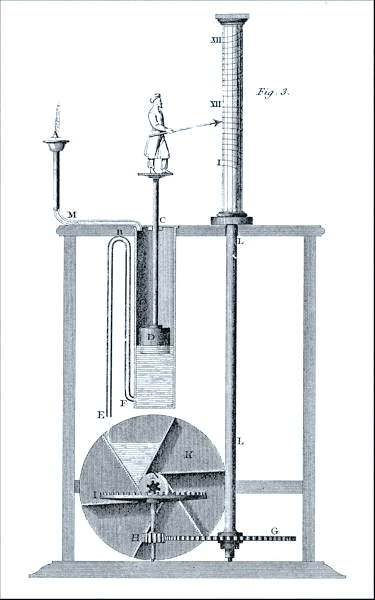
\includegraphics[height=4.5cm]{water_clock_ctesibius.jpg}

\smallskip
{\scriptsize Ktesibios' water clock.\par}
\end{column}
\begin{column}{0.48\textwidth}
\footnotesize
\begin{minipage}[t][2.9cm][t]{\linewidth}
\raggedright
\alert{18th century.} In 1788 James Watt fits a \emph{centrifugal governor} to the steam engine. As the engine speeds up, the two rotating balls move outward and close the steam valve; as it slows down, they fall and open it.
\end{minipage}

\medskip
\centering
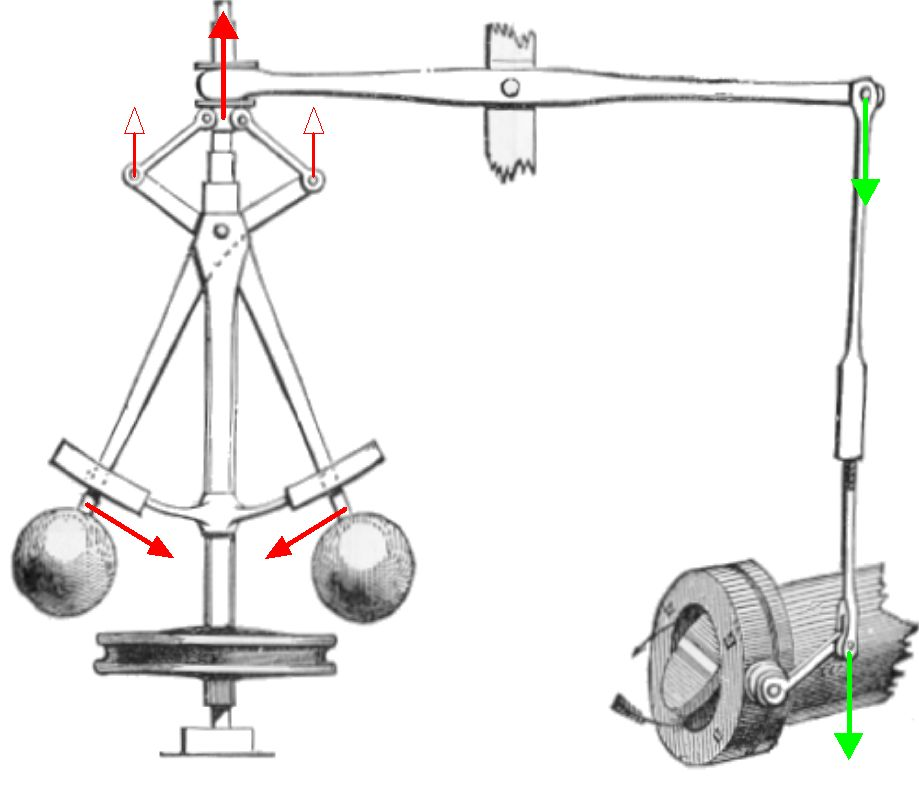
\includegraphics[height=4.5cm]{governor_watt_diagram.jpg}

\smallskip
{\scriptsize Watt's governor and steam valve.\par}
\end{column}
\end{columns}
% \medskip
% \alert{The pattern.} A quantity is \emph{measured} (a water level, a speed), compared with what is wanted, and the difference \emph{acts back} on the system. These devices worked for decades before anyone could say when they work.
\end{frame}


% =========================================================================
\begin{frame}{Maxwell, 1868: \emph{On Governors}}
\begin{columns}[T]
\begin{column}{0.50\textwidth}
\footnotesize
Maxwell studied why a governor can fail to settle at a steady speed and instead oscillate \citep{maxwell1868}.
\begin{itemize}
\item For small deviations, use a \alert{linear differential equation}.
% \item Its modes are $e^{\lambda t}$, where $\lambda$ solves a \alert{characteristic polynomial}.
\item Disturbances decay if \alert{every root has negative real part}. Complex roots with positive real part make oscillations grow.
\end{itemize}
Routh (1877) and Hurwitz (1895) later developed a general stability test.

\end{column}
\begin{column}{0.47\textwidth}
\centering
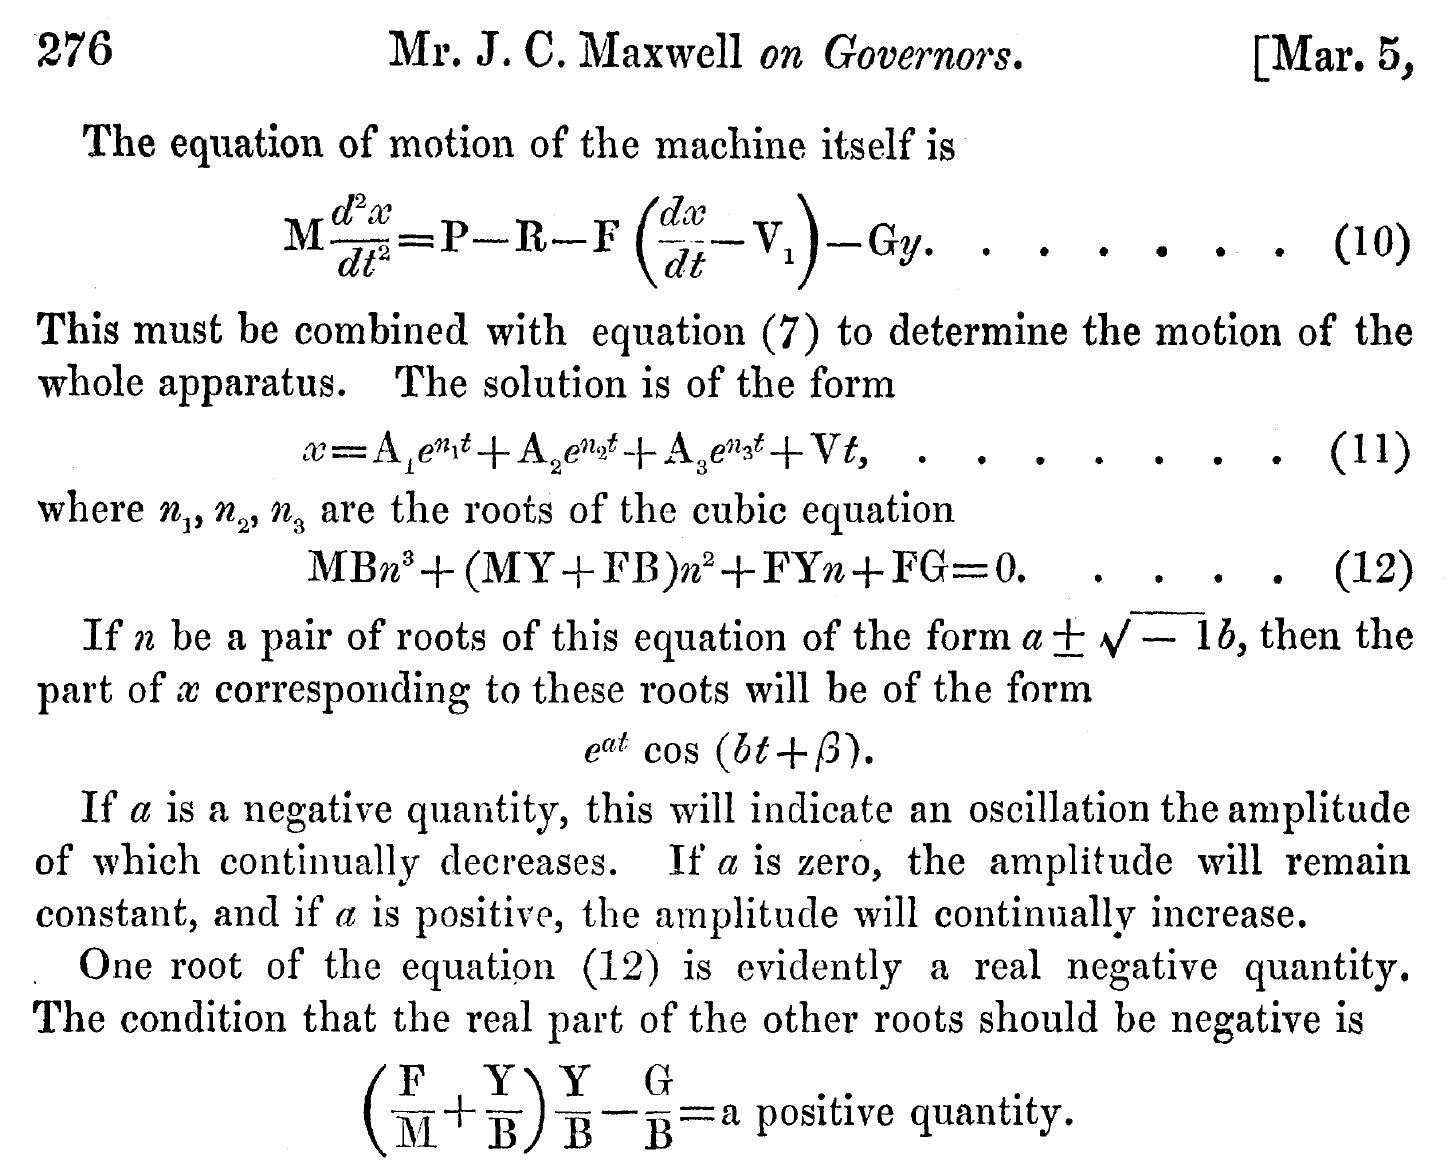
\includegraphics[width=\textwidth]{maxwell_1868_equations.png}

\smallskip
\scriptsize \href{https://webhomes.maths.ed.ac.uk/~v1ranick/papers/maxwell1.pdf}{\emph{On Governors} (1868), p.~276.}\\
The original equation, exponential modes and stability condition.
\end{column}
\end{columns}
\end{frame}


% =========================================================================
\begin{frame}{A timeline}
\begin{center}
\resizebox{\textwidth}{!}{%
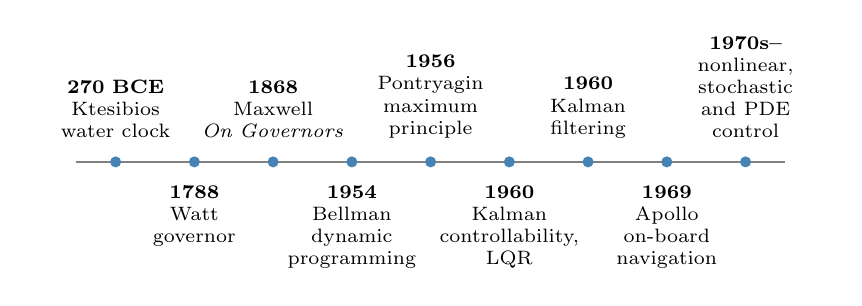
\begin{tikzpicture}[every node/.style={font=\scriptsize}]
  \draw[gray, line width=0.8pt] (-0.5,0) -- (8.5,0);
  \foreach \x/\yr/\txt/\anc/\dy in {
     0/270 BCE/{Ktesibios\\water clock}/south/0.18,
     1/1788/{Watt\\governor}/north/-0.18,
     2/1868/{Maxwell\\\emph{On Governors}}/south/0.18,
     3/1954/{Bellman\\dynamic programming}/north/-0.18,
     4/1956/{Pontryagin\\maximum principle}/south/0.18,
     5/1960/{Kalman\\controllability, LQR}/north/-0.18,
     6/1960/{Kalman\\filtering}/south/0.18,
     7/1969/{Apollo\\on-board navigation}/north/-0.18,
     8/1970s--/{nonlinear, stochastic\\and PDE control}/south/0.18}
  {
    \fill[boxframe] (\x,0) circle (2pt);
    \node[anchor=\anc, align=center, text width=2cm] at (\x,\dy) {\textbf{\yr}\\\txt};
  }
\end{tikzpicture}}
\end{center}

% \bigskip
% \small
% Two parallel languages grew during the 20th century: the \alert{frequency domain} (Fourier, transfer functions, Bode and Nyquist plots: the engineer's language) and the \alert{state space} (differential equations and matrices: the language of this course). Kalman's work of 1960 made the second one complete for linear systems.
\end{frame}


% =========================================================================
% \begin{frame}{From feedback to state space}
% \footnotesize
% \begin{itemize}
% \item \alert{1920s--30s.} Feedback enters telecommunications at the Bell Laboratories: Black's negative-feedback amplifier (1927) trades gain for precision and robustness; Nyquist (1932) and Bode give stability criteria in the frequency domain. Automatic control spreads to industry, then to aircraft and fire control.
% \item \alert{1948.} Wiener names the field: \emph{Cybernetics}, ``the science of control and communication in the animal and the machine'' \citep{wiener1948}.
% \item \alert{1950s--60s.} Bellman's dynamic programming \citep{bellman1954}, Pontryagin's maximum principle \citep{pontryagin1962}, a far-reaching generalization of Lagrange multipliers, and Kalman's work \citep{kalman1960} establish modern \emph{state-space} control. Kalman introduces \alert{controllability} and \alert{observability} and analyzes the linear--quadratic regulator with a Riccati equation.
% \item \alert{1960.} Kalman's filter \citep{kalman1960filter} addresses a different task, estimating the state from noisy measurements; it was used in Apollo's on-board navigation.
% \item \alert{Since then.} Nonlinear, stochastic and infinite-dimensional (PDE) systems, with applications from acoustics and quantum control to aerospace, biomedicine and energy, and, as we shall see, machine learning.
% \end{itemize}
% \end{frame}


% =========================================================================
\section{Dynamical systems}

\begin{frame}{What is a dynamical system?}
A \alert{dynamical system} is a state space $X$ together with a rule for how the state changes over time.

\medskip
In \alert{discrete time}, one map gives one step:
\[
F:X\to X,\qquad x_{k+1}=F(x_k),\qquad k=0,1,2,\ldots
\]
\small
\begin{itemize}
\item The \alert{state} records what we need to know now to predict what happens later. %For a mass, it is position and velocity; for a heated bar, the temperature profile.
% \item Starting from $x_0$, repeat the rule: $x_0,x_1,x_2,\ldots$ is a \alert{trajectory}.
\item In \alert{continuous time}, the rule is usually a differential equation, $x'=f(x)$.
\item A map $F$ gives a \alert{deterministic} update. A \alert{stochastic} system uses transition probabilities instead.
\end{itemize}

\end{frame}


% =========================================================================
\begin{frame}{Discrete time, finite state set}
\footnotesize
$X$ is finite. Each step follows a \alert{deterministic rule} or \alert{transition probabilities}.

\medskip
\begin{columns}[T,onlytextwidth]
\begin{column}{0.31\textwidth}
\alert{\textbf{A traffic light}}

\smallskip
\begin{minipage}[c][2.4cm][c]{\linewidth}
\centering
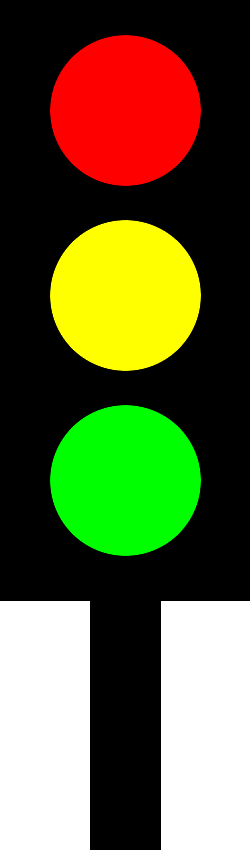
\includegraphics[height=2.2cm]{traffic_light.png}
\end{minipage}

\smallskip
The state is the active light: green, yellow or red.
\[
X=\{G,Y,R\}.
\]
In a simplified cycle, $F$ advances to the next light:
\[
G\to Y\to R\to G.
\]
\end{column}
\begin{column}{0.31\textwidth}
\alert{\textbf{A magnet: Ising spins}}

\smallskip
\begin{minipage}[c][2.4cm][c]{\linewidth}
\centering
\resizebox{\linewidth}{!}{% Four classical Ising spins before and after one accepted spin flip.
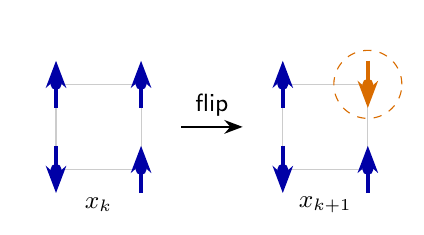
\begin{tikzpicture}[>=Stealth, x=6mm, y=6mm, font=\sffamily\small]
  \path[use as bounding box] (-0.6,-0.8) rectangle (7.2,3.0);
  \foreach \offset in {0,4.8} {
    \draw[black!20] (\offset,0) rectangle ++(1.8,1.8);
  }
  \foreach \x/\y/\spin in {0/0/-1,0/1.8/1,1.8/0/1,1.8/1.8/1} {
    \fill[blue!65!black] (\x,\y) circle (2pt);
    \draw[->,blue!65!black,line width=1.5pt]
      (\x,{\y-0.5*\spin}) -- (\x,{\y+0.5*\spin});
  }
  \foreach \x/\y/\spin in {4.8/0/-1,4.8/1.8/1,6.6/0/1} {
    \fill[blue!65!black] (\x,\y) circle (2pt);
    \draw[->,blue!65!black,line width=1.5pt]
      (\x,{\y-0.5*\spin}) -- (\x,{\y+0.5*\spin});
  }
  \draw[orange!85!black,dashed] (6.6,1.8) circle (0.72);
  \fill[orange!85!black] (6.6,1.8) circle (2pt);
  \draw[->,orange!85!black,line width=1.5pt] (6.6,2.3) -- (6.6,1.3);
  \draw[->,thick] (2.65,0.9) -- node[above] {flip} (3.95,0.9);
  \node at (0.9,-0.75) {$x_k$};
  \node at (5.7,-0.75) {$x_{k+1}$};
\end{tikzpicture}
}
\end{minipage}

\smallskip
$N$ spins, each pointing up or down:
\[
X=\{-1,+1\}^{N}.
\]
One step attempts a spin flip; its acceptance probability depends on the energy change.
\end{column}
\begin{column}{0.31\textwidth}
\alert{\textbf{A Markov chain}}

\smallskip
\begin{minipage}[c][2.4cm][c]{\linewidth}
\centering
\resizebox{\linewidth}{!}{% Illustrative two-state weather chain; outgoing probabilities sum to one.
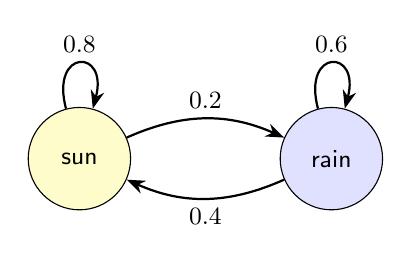
\begin{tikzpicture}[>=Stealth, font=\sffamily\small,
  state/.style={circle,draw,minimum size=13mm,inner sep=1pt}]
  \node[state,fill=yellow!20] (sun) at (0,0) {sun};
  \node[state,fill=blue!12] (rain) at (3.2,0) {rain};
  \draw[->,thick] (sun) to[bend left=24] node[above] {$0.2$} (rain);
  \draw[->,thick] (rain) to[bend left=24] node[below] {$0.4$} (sun);
  \draw[->,thick] (sun) to[loop above,looseness=6] node[above] {$0.8$} (sun);
  \draw[->,thick] (rain) to[loop above,looseness=6] node[above] {$0.6$} (rain);
\end{tikzpicture}
}
\end{minipage}

\smallskip
The next state is random, with probabilities depending only on the current state.
\[
p_{k+1}=P^{\!\top}p_k.
\]
$p_k$ is the probability vector over $X$; $P$ is the transition matrix.
\end{column}
\end{columns}
\end{frame}


% =========================================================================
\begin{frame}{Discrete time in $\R^n$}
\footnotesize
The state is a \alert{vector}; each step applies an update map, $x_{k+1}=f_k(x_k)$.

\medskip
\begin{columns}[T,onlytextwidth]
\begin{column}{0.31\textwidth}
\alert{\textbf{The logistic map}}

\smallskip
\begin{minipage}[c][2.4cm][c]{\linewidth}
\centering
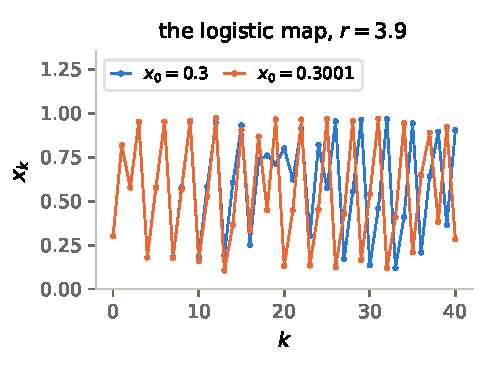
\includegraphics[width=\linewidth]{ds_discrete.pdf}
\end{minipage}

\smallskip
The state is a population with limited resources:
\[
x_{k+1}=r\,x_k(1-x_k).
\]
The two initial states shown differ by $10^{-4}$.
\end{column}
\begin{column}{0.31\textwidth}
\alert{\textbf{A residual network}}

\smallskip
\begin{minipage}[c][2.4cm][c]{\linewidth}
\centering
\resizebox{\linewidth}{!}{% One residual layer: the identity branch adds a learned increment h g_k(x_k).
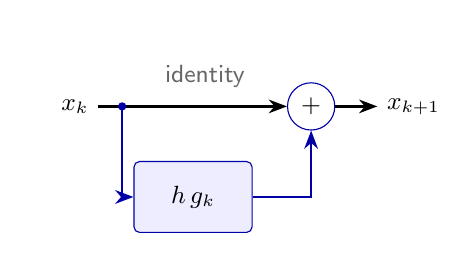
\begin{tikzpicture}[>=Stealth, font=\sffamily\small,
  transform/.style={draw=blue!65!black,fill=blue!7,rounded corners=2pt,
    minimum width=15mm,minimum height=9mm}]
  \path[use as bounding box] (-0.6,-1.6) rectangle (4.6,1.0);
  \node (input) at (0,0) {$x_k$};
  \node[circle,draw=blue!65!black,minimum size=6mm,inner sep=0pt] (sum) at (3,0) {$+$};
  \node (output) at (4.3,0) {$x_{k+1}$};
  \node[transform] (increment) at (1.5,-1.15) {$h\,g_k$};
  \coordinate (branch) at (0.6,0);
  \draw[->,thick] (input) -- (sum);
  \fill[blue!65!black] (branch) circle (1.5pt);
  \draw[->,thick,blue!65!black] (branch) |- (increment);
  \draw[->,thick,blue!65!black] (increment) -| (sum);
  \draw[->,thick] (sum) -- (output);
  \node[above,text=black!60] at (1.65,0.12) {identity};
\end{tikzpicture}
}
\end{minipage}

\smallskip
The state is a data point's features. Each layer adds a learned increment:
\[
\begin{aligned}
x_{k+1}&=x_k+h\,g_k(x_k),
\end{aligned}
\]
where $g_k$ is a neural network and $h>0$ is a step size.
\end{column}
\begin{column}{0.31\textwidth}
\alert{\textbf{Gradient descent}}

\smallskip
\begin{minipage}[c][2.4cm][c]{\linewidth}
\centering
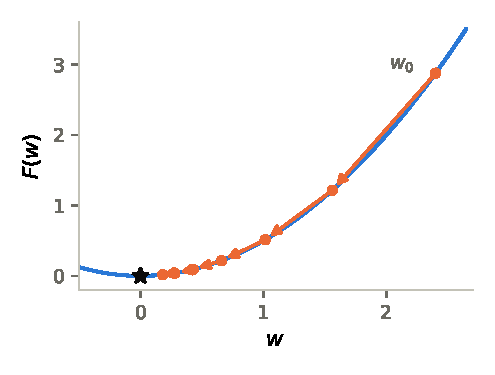
\includegraphics[width=\linewidth]{ds_gradient_descent.pdf}
\end{minipage}

\smallskip
The state is the parameter vector; $F$ is the loss:
\[
w_{k+1}=w_k-\eta\,\nabla F(w_k).
\]
The step size is $\eta>0$.
\end{column}
\end{columns}
\end{frame}


% =========================================================================
\begin{frame}{Continuous time in $\R^n$}
\footnotesize
The state evolves continuously, following a \alert{deterministic} or \alert{stochastic} rule.

\medskip
\begin{columns}[T,onlytextwidth]
\begin{column}{0.31\textwidth}
\alert{\textbf{Newton's law}}

\smallskip
\begin{minipage}[c][2.4cm][c]{\linewidth}
\centering
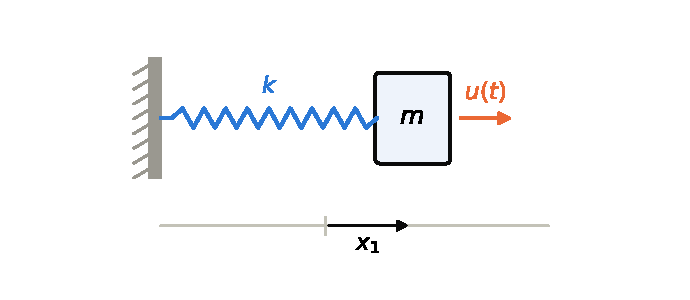
\includegraphics[width=\linewidth]{spring_mass.pdf}
\end{minipage}

\smallskip
Position and velocity form the state $x=(q,v)$:
\[
q'=v,\quad m\,v'=F(q,v).
\]
% Given the initial state, the ODE determines the motion.
\end{column}
\begin{column}{0.31\textwidth}
\alert{\textbf{The pendulum}}

\smallskip
\begin{minipage}[c][2.4cm][c]{\linewidth}
\centering
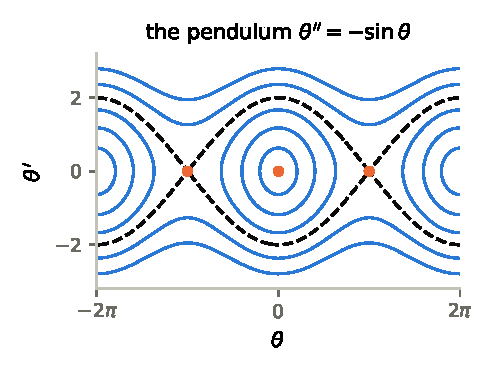
\includegraphics[width=\linewidth]{ds_pendulum.pdf}
\end{minipage}

\smallskip
The state is angle and angular velocity, $x=(\theta,\theta')$:
\[
\theta''=-\sin\theta.
\]
% Energy is conserved; the phase-plane orbits are its level sets.
\end{column}
\begin{column}{0.31\textwidth}
\alert{\textbf{Brownian motion}}

\smallskip
\begin{minipage}[c][2.4cm][c]{\linewidth}
\centering
% The GIF and these vector PDF frames are generated by make_figures.py.
% A complete trajectory remains visible in PDF viewers without animation support.
\animategraphics[autoplay,loop,poster=last,width=\linewidth]{20}{images/brownian_motion}{}{}
\end{minipage}

\smallskip
A particle's position is random, $X_t\in\R^2$:
\[
dX_t=dW_t,\qquad X_0=0.
\]
% Paths are continuous, almost surely nowhere differentiable: this is a stochastic evolution.
\end{column}
\end{columns}
\end{frame}


% =========================================================================
\begin{frame}{Infinite dimension: partial differential equations}
\footnotesize
The state is a \alert{function} of space; its evolution follows a PDE.

\medskip
\begin{columns}[T,onlytextwidth]
\begin{column}{0.31\textwidth}
\alert{\textbf{Heat}}

\smallskip
\begin{minipage}[c][2.4cm][c]{\linewidth}
\centering
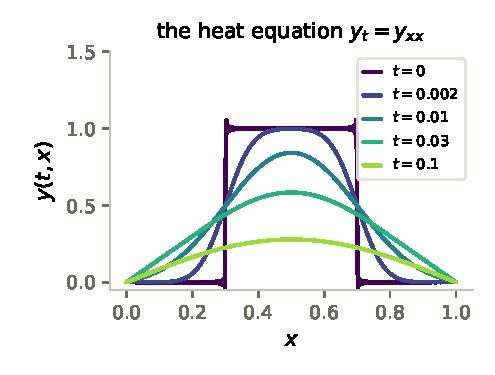
\includegraphics[width=\linewidth]{ds_heat.pdf}
\end{minipage}

\smallskip
The state is the temperature profile $y(t,\cdot)\in L^2(0,1)$:
\[
\begin{gathered}
y_t=y_{xx},\\
y(t,0)=y(t,1)=0.
\end{gathered}
\]
Diffusion smooths the profile.
\end{column}
\begin{column}{0.31\textwidth}
\alert{\textbf{Waves}}

\smallskip
\begin{minipage}[c][2.4cm][c]{\linewidth}
\centering
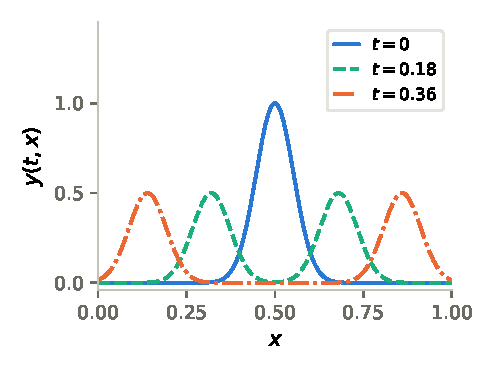
\includegraphics[width=\linewidth]{ds_wave.pdf}
\end{minipage}

\smallskip
Displacement and velocity form the state $(y,y_t)$:
\[
y_{tt}=y_{xx}.
\]
A pulse splits into two waves travelling in opposite directions.
\end{column}
\begin{column}{0.31\textwidth}
\alert{\textbf{Transport}}

\smallskip
\begin{minipage}[c][2.4cm][c]{\linewidth}
\centering
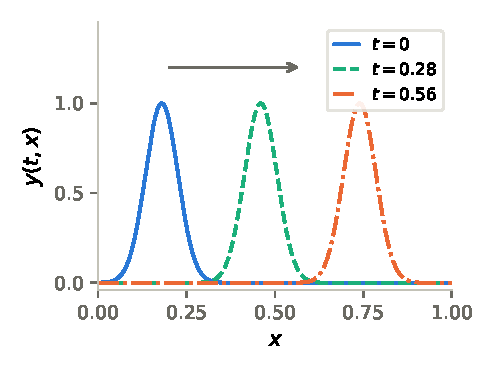
\includegraphics[width=\linewidth]{ds_transport.pdf}
\end{minipage}

\smallskip
The state is a moving profile $y(t,\cdot)$:
\[
\begin{gathered}
y_t+c\,y_x=0,\\
y(t,x)=y_0(x-ct).
\end{gathered}
\]
The shape moves at speed $c$.
\end{column}
\end{columns}
\end{frame}


% =========================================================================
\begin{frame}{Dynamical systems: summary}
\renewcommand{\arraystretch}{1.3}
\footnotesize
\begin{tabular}{@{}p{0.24\textwidth} p{0.28\textwidth} p{0.42\textwidth}@{}}
\toprule
\textbf{Time, state space} & \textbf{Rule} & \textbf{Examples} \\
\midrule
discrete, $X$ finite & $x_{k+1}=F(x_k)$ & traffic light, board game; a Markov chain on the probabilities \\
discrete, $X=\R^n$ & $x_{k+1}=f(x_k)$ & logistic map; Euler's method; a residual network; gradient descent \\
continuous, $X=\R^n$ & $x'=f(x)$ or $dX=dW$ & Newton's law; pendulum; Brownian motion \\
continuous, $X$ infinite dimensional & $y_t=\Delta y$, \ $y_{tt}=\Delta y$, \ $y_t+c\,y_x=0$ & heat, waves, transport \\
\bottomrule
\end{tabular}

% \bigskip
% \small
% Also \alert{stochastic} rules, $x_{k+1}=f(x_k,\xi_k)$ with random $\xi_k$ or $dX=f(X)\,dt+\sigma(X)\,dW$, and \alert{hybrid} ones mixing discrete and continuous evolution (a bouncing ball, a thermostat with a switch).

% \medskip
% \alert{Preview.} A residual network is a discrete dynamical system whose rule is \emph{learned}, and a neural ODE is its continuous-time limit. The dynamical point of view on machine learning is the thread of this course.
\end{frame}


% =========================================================================
\section{Dynamical systems with control}

\begin{frame}{Dynamical systems: adding a control}
A control is an \alert{input $u$ that we choose} to influence the evolution.

\medskip
\begin{columns}[T,onlytextwidth]
\begin{column}{0.47\textwidth}
\alert{\textbf{Without control}}


\[
x'(t)=f\big(x(t)\big).
\]
\end{column}
\begin{column}{0.47\textwidth}
\alert{\textbf{With control}}

\[
x'(t)=f\big(x(t),u(t)\big).
\]
\end{column}
\end{columns}
\end{frame}


% =========================================================================
\begin{frame}{Control systems: three examples}
\footnotesize
Three of the systems from before, now with an input $\ctrl{u}$ that we choose.

\medskip
\begin{columns}[T,onlytextwidth]
\begin{column}{0.31\textwidth}
\alert{\textbf{The pendulum}}

\smallskip
\begin{minipage}[c][2.4cm][c]{\linewidth}
\centering
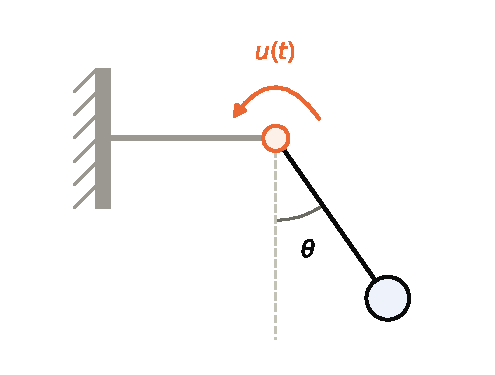
\includegraphics[width=\linewidth]{ctrl_pendulum.pdf}
\end{minipage}

\smallskip
A motor at the pivot applies a torque $\ctrl{u(t)}$:
\[
\theta''=-\sin\theta+\ctrl{u}.
\]
A feedback $\ctrl{u}(\theta,\theta')$ can hold the pendulum upright, at $\theta=\pi$.
\end{column}
\begin{column}{0.31\textwidth}
\alert{\textbf{A residual network}}

\smallskip
\begin{minipage}[c][2.4cm][c]{\linewidth}
\centering
\resizebox{\linewidth}{!}{% One residual layer with its parameters drawn as the control u_k = (W_k, b_k).
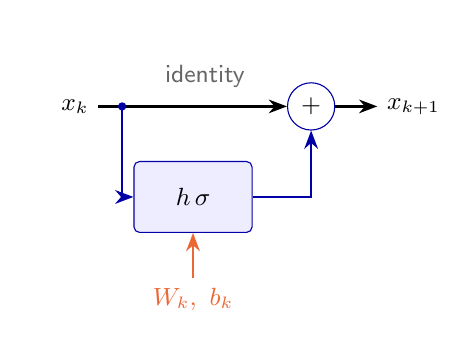
\begin{tikzpicture}[>=Stealth, font=\sffamily\small,
  transform/.style={draw=blue!65!black,fill=blue!7,rounded corners=2pt,
    minimum width=15mm,minimum height=9mm}]
  \path[use as bounding box] (-0.6,-2.75) rectangle (4.6,1.0);
  \node (input) at (0,0) {$x_k$};
  \node[circle,draw=blue!65!black,minimum size=6mm,inner sep=0pt] (sum) at (3,0) {$+$};
  \node (output) at (4.3,0) {$x_{k+1}$};
  \node[transform] (increment) at (1.5,-1.15) {$h\,\sigma$};
  \node[text=ctrl] (weights) at (1.5,-2.45) {$W_k,\ b_k$};
  \coordinate (branch) at (0.6,0);
  \draw[->,thick] (input) -- (sum);
  \fill[blue!65!black] (branch) circle (1.5pt);
  \draw[->,thick,blue!65!black] (branch) |- (increment);
  \draw[->,thick,blue!65!black] (increment) -| (sum);
  \draw[->,thick,ctrl] (weights) -- (increment);
  \draw[->,thick] (sum) -- (output);
  \node[above,text=black!60] at (1.65,0.12) {identity};
\end{tikzpicture}
}
\end{minipage}

\smallskip
Each layer has weights and a bias; $\sigma$ is a fixed activation:
\[
\mathclap{x_{k+1}=x_k+h\,\sigma(\ctrl{W_k}x_k+\ctrl{b_k}).}
\]
Training chooses $\ctrl{u_k}=(\ctrl{W_k},\ctrl{b_k})$; the same control acts on every data point.
\end{column}
\begin{column}{0.31\textwidth}
\alert{\textbf{Heat}}

\smallskip
\begin{minipage}[c][2.4cm][c]{\linewidth}
\centering
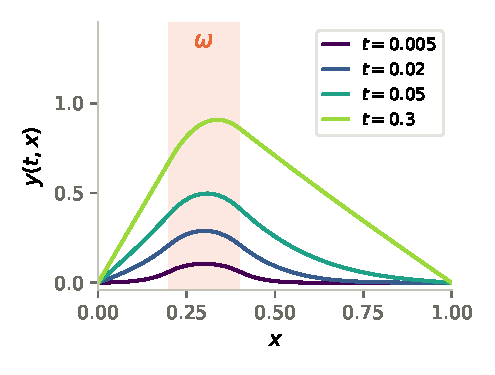
\includegraphics[width=\linewidth]{ctrl_heat.pdf}
\end{minipage}

\smallskip
A heater acts only on a subregion $\omega\subset(0,1)$:
\[
\begin{gathered}
y_t=y_{xx}+\mathbf{1}_\omega\,\ctrl{u},\\
y(t,0)=y(t,1)=0.
\end{gathered}
\]
Here $\ctrl{u}$ is constant and $y(0,\cdot)=0$: heat enters through $\omega$, then spreads.
\end{column}
\end{columns}
\end{frame}


% =========================================================================
% \begin{frame}{Control systems: states and inputs}
% \renewcommand{\arraystretch}{1.3}
% \footnotesize
% \begin{tabularx}{\textwidth}{@{}p{0.23\textwidth} p{0.40\textwidth} X@{}}
% \toprule
% \textbf{System} & \textbf{State $x$} & \textbf{Control $u$} \\
% \midrule
% pendulum, crane, rocket & angle and angular velocity; position and velocity & torque; force; thrust \\
% a heated room & temperature deviation: $x'=-x+u+d$ & heating power ($d$: an unknown disturbance) \\
% inventory & stock: $x_{k+1}=x_k+u_k-d_k$ & orders ($d_k$: the demand) \\
% heat in a domain $\Omega$ & temperature field $y(t,\cdot)$ & a heater acting on a subregion $\omega\subset\Omega$ \\
% residual network & the features of a data point & the weights of each layer \\
% \bottomrule
% \end{tabularx}

% \medskip
% \small
% The control enters where we can act: a motor, a valve, a heater, a parameter. Usually there are far fewer controls than state variables.
% \end{frame}


% =========================================================================
\begin{frame}{The ingredients of a control problem}
\begin{enumerate}
\item \alert{A state equation}, which describes how the state evolves and where we can act. For most of the course,
\[
x'(t)=f\big(x(t),u(t)\big),\quad t\in(0,T),\qquad x(0)=x^0,
\]
with the \textbf{state} $x(t)\in\R^n$ and the \textbf{control} $u(t)\in\R^m$.
\item \alert{A set of admissible controls} $\Uad$ the control is taken from. Typical choices: $\Uad=L^2(0,T;\R^m)$, finite energy; or controls with bounds.
\item \alert{An objective}: a target to reach, a cost to minimize, or an equilibrium to keep. 
\end{enumerate}

% \medskip
% The same framework covers very different models: linear or nonlinear, deterministic or stochastic, finite- or infinite-dimensional, ordinary or partial differential equations, as well as hybrid models. What changes from one to the other is the \emph{answer}, not the question.
\end{frame}


% =========================================================================
\begin{frame}{From nonlinear to linear: linearization}
Let $(\bar x,\bar u)$ be an equilibrium, $f(\bar x,\bar u)=0$, and write $x=\bar x+\xi$, $u=\bar u+v$. Taylor's formula gives
\[
\xi'=f(\bar x+\xi,\bar u+v)=\underbrace{D_xf(\bar x,\bar u)}_{A}\,\xi+\underbrace{D_uf(\bar x,\bar u)}_{B}\,v+O\big(|\xi|^2+|v|^2\big).
\]
To first order the system is \alert{linear and time-invariant}: $\xi'=A\xi+Bv$. This is what Maxwell did with the governor, and what every engineer does first.

% \medskip
% \alert{Example: the pendulum with a torque,} $\theta''=-\sin\theta+u$. State $x=(\theta,\theta')$, $f(x,u)=(x_2,\,-\sin x_1+u)$.
% \begin{itemize}
% \item Hanging down, $\bar x=(0,0)$: $A=\begin{pmatrix}0&1\\-1&0\end{pmatrix}$, $B=\begin{pmatrix}0\\1\end{pmatrix}$: the \textbf{harmonic oscillator} $\xi_1''+\xi_1=v$.
% \item Standing up, $\bar x=(\pi,0)$: $A=\begin{pmatrix}0&1\\1&0\end{pmatrix}$, eigenvalues $\pm1$: \textbf{unstable}. Keeping it there is a feedback problem.
% \end{itemize}
% \alert{Why it matters.} If the linearization is controllable, the nonlinear system is controllable near the equilibrium (small displacements, small controls): linear theory is the local theory of everything.
\end{frame}


% =========================================================================
\section{Linear systems and the harmonic oscillator}

\begin{frame}{The linear time-invariant setting}
Let $n,m\ge1$ and $T>0$. We study
\[
x'(t)=Ax(t)+Bu(t),\quad t\in(0,T),\qquad x(0)=x^0,
\]
with $A\in\R^{n\times n}$ and $B\in\R^{n\times m}$. The state has $n$ components and the control $m$. %In practice $m\le n$, often $m\ll n$: \alert{control as much as possible with as few controls as possible.}

\medskip
\begin{mathbox}{Variation of constants}
\[
x(t)=e^{At}x^0+\int_0^te^{A(t-s)}Bu(s)\,ds .
\]
\end{mathbox}
\emph{Proof.} Multiply the equation by $e^{-At}$: $\big(e^{-At}x(t)\big)'=e^{-At}\big(x'(t)-Ax(t)\big)=e^{-At}Bu(t)$. Integrate from $0$ to $t$ and multiply by $e^{At}$. \hfill$\square$

% \medskip
% The state at time $t$ is the \alert{free evolution} $e^{At}x^0$ plus a contribution that is \alert{linear in the control}. Everything in this lecture follows from this formula.
\end{frame}


% =========================================================================
\begin{frame}{Example: the harmonic oscillator}
\begin{columns}[T]
\begin{column}{0.5\textwidth}
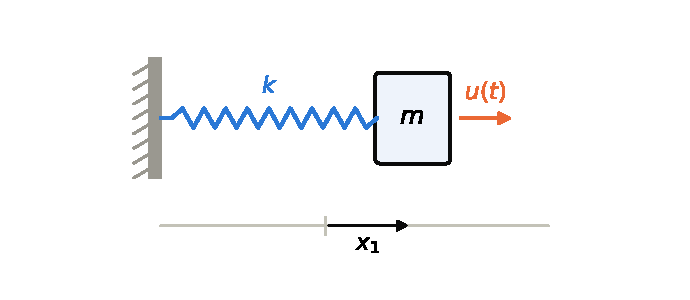
\includegraphics[width=0.92\textwidth]{spring_mass.pdf}
\end{column}
\begin{column}{0.5\textwidth}
\small
A mass $m_0$ attached to a spring of stiffness $k$, pushed by a force $u(t)$. Newton's law:
\[
m_0\,q''=-k\,q+u .
\]
\end{column}
\end{columns}
\small
With the state $x=(x_1,x_2)=(q,q')$, position and velocity, one second-order equation becomes two first-order ones:
\[
x'=\underbrace{\begin{pmatrix}0&1\\-k/m_0&0\end{pmatrix}}_{A}x+\underbrace{\begin{pmatrix}0\\1/m_0\end{pmatrix}}_{B}u .
\]
\end{frame}


% =========================================================================
% \begin{frame}{The free oscillator, and a first feedback}
% \begin{center}
% 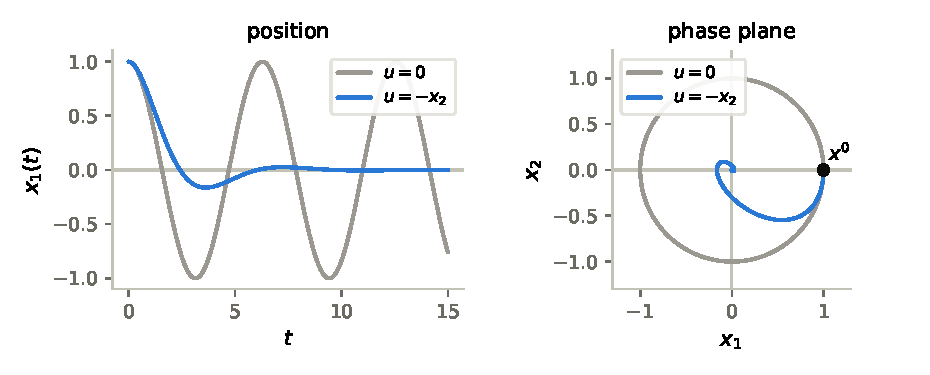
\includegraphics[width=0.78\textwidth]{oscillator_free_feedback.pdf}
% \end{center}
% \footnotesize
% \alert{No control.} From $x^0=(1,0)$, $x(t)=(\cos t,-\sin t)$: the energy $e=\tfrac12(x_1^2+x_2^2)$ is conserved and the state runs around a circle forever.

% \alert{Friction.} $u=-x_2$ gives $x_1''+x_1'+x_1=0$. Along solutions $e'=x_1x_1'+x_2x_2'=x_2(x_1-x_1-x_2)=-x_2^2\le0$: the energy decreases and the state spirals to rest.

% \alert{Is friction a control?} It is a \emph{feedback}: $u$ is computed from the current state by the rule $F(x)=-x_2$. A damper does it mechanically; a motor reading a velocity sensor does the same.
% \nbref{01 \S4}
% \end{frame}


% =========================================================================
\section{Three questions}

\begin{frame}{Three different questions}
Several kinds of control problems fit the same framework, depending on how the objective is formulated.

\medskip
\footnotesize
\begin{columns}[T,onlytextwidth]
\begin{column}{0.31\textwidth}
\alert{\textbf{Controllability}}

\smallskip
Given $x^0$, $x^1$ and $T$: is there $u\in\Uad$ such that
\[
x(T)=x^1\,?
\]
A dynamical notion: can the target be \emph{reached}? 
\end{column}
\hfill
\begin{column}{0.35\textwidth}
\alert{\textbf{Optimal control}}

\smallskip
Find which $u\in\Uad$ minimizes a cost, for instance
\[
J(u)=|x(T)-x^1|^2+\!\int_0^T\!|u|^2dt
\]
It need not reach the target: it makes the best compromise allowed by the cost.
\end{column}
\hfill
\begin{column}{0.31\textwidth}
\alert{\textbf{Stabilization}}

\smallskip
Is there a \emph{rule} $u=F(x)$ such that every solution of
\[
x'=f\big(x,F(x)\big)
\]
tends to an equilibrium?
\end{column}
\end{columns}

\medskip
\begin{columns}[T,onlytextwidth]
\begin{column}{0.31\textwidth}
\centering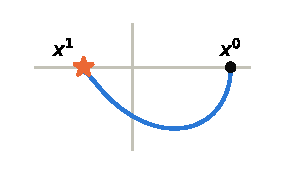
\includegraphics[width=\textwidth]{three_questions_controllability.pdf}
\end{column}
\hfill
\begin{column}{0.35\textwidth}
\centering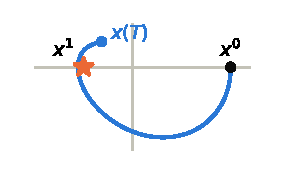
\includegraphics[width=0.886\textwidth]{three_questions_optimal.pdf}
\end{column}
\hfill
\begin{column}{0.31\textwidth}
\centering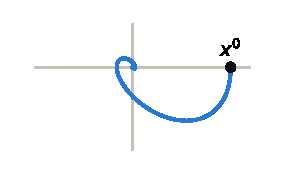
\includegraphics[width=\textwidth]{three_questions_stabilization.pdf}
\end{column}
\end{columns}

\end{frame}


% =========================================================================
\begin{frame}{Open loop and closed loop}
\begin{columns}[T]
\begin{column}{0.5\textwidth}
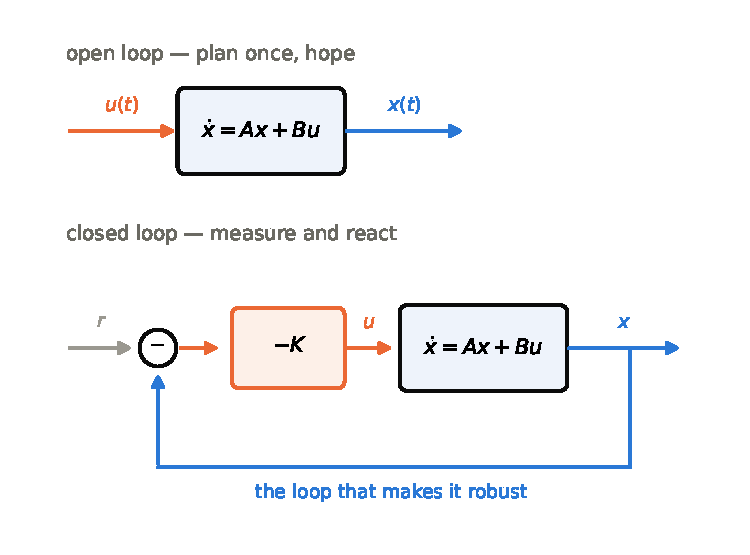
\includegraphics[width=\textwidth]{feedback_diagram.pdf}
\end{column}
\begin{column}{0.5\textwidth}
\footnotesize
The last question introduces a distinction that runs through the whole course. A control can be
\begin{enumerate}
\item \alert{open loop}, $u=u(t)$: a function of time, computed in advance from the model and then applied blindly;
\item \alert{closed loop} or \alert{feedback}, $u=F(x(t))$: computed in real time from the current state, so it can react to disturbances the model does not know about.
\end{enumerate}

% \medskip
% In a feedback process the state of the system determines the way the control is exerted: the cause--effect principle becomes a \emph{cause--effect--cause} principle.

% \medskip
% Controllability and optimal control, as posed, produce open-loop controls; stabilization asks for a feedback. Later lectures show how the two are linked.
\end{column}
\end{columns}
\end{frame}


% =========================================================================
\begin{frame}{Why feedback? A thermostat}
\begin{columns}[T]
\begin{column}{0.56\textwidth}
\footnotesize
Temperature deviation $x$, heating $u$, setpoint $1$, and an \emph{unknown} constant disturbance $d$ (an open window):
\[
x'=-x+u+d,\qquad x(0)=0 .
\]
\alert{Open loop.} The model says $u\equiv1$ brings $x$ to $1$. With the disturbance, $x(t)\to1+d$: the error is the full disturbance.

\alert{Feedback.} $u=1+L\,(1-x)$ with gain $L>0$. Then $x'=-(1+L)x+1+L+d$ and
\[
x(t)\to1+\frac{d}{1+L}\qquad\text{as }t\to\infty .
\]
The error shrinks like $1/(1+L)$, \emph{without knowing} $d$, and the response is faster.

% \alert{The price.} If the sensor is biased, reading $x+\beta$ instead of $x$, the limit is $1+\frac{d}{1+L}-\frac{L\beta}{1+L}$: a large gain trusts the measurement completely. Feedback trades model error for measurement error.
\end{column}
\begin{column}{0.44\textwidth}
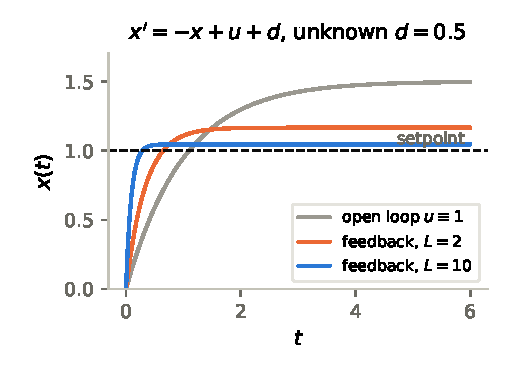
\includegraphics[width=\textwidth]{thermostat.pdf}

% \scriptsize Open loop and two feedback gains for the same unknown disturbance.
\end{column}
\end{columns}
\end{frame}


% =========================================================================
\begin{frame}{Feedback everywhere}
\footnotesize
The concept of feedback comes from the capacity of biological systems to regulate themselves, and was incorporated into control engineering in the 1920s.

\medskip
\begin{columns}[T]
\begin{column}{0.48\textwidth}
\alert{Engineering}
\begin{itemize}
\item thermostats, cruise control, autopilots
\item the governor, and the hunting it may cause
\item active noise cancelling: measure the sound, emit the opposite
\item robots, rockets, chemical reactors, power grids
\end{itemize}
\end{column}
\begin{column}{0.52\textwidth}
\alert{Nature and learning}
\begin{itemize}
\item homeostasis: body temperature, glucose, blood pressure
\item a cyclist balancing, a hand reaching for a cup
\item reinforcement learning: an action depends on the observed state; the policy is \emph{learned} from rewards instead of \emph{designed} from a model
\item gradient descent with momentum
\end{itemize}
\end{column}
\end{columns}


\end{frame}


% =========================================================================
\begin{frame}{Part I: key takeaways}
\begin{enumerate}
\item A dynamical system is a state space and an evolution rule: $x_{k+1}=F(x_k)$ in discrete time, or a differential equation in continuous time.
\item A control problem consists of a state equation, a set of admissible controls and an objective.

\item Controllability: \emph{can} the target be reached? Optimal control: which admissible control is \emph{best}? Stabilization: is there a \emph{rule} $u=F(x)$ that makes the equilibrium attracting?
\item Open loop: $u=u(t)$, computed in advance. Closed loop: $u=F(x(t))$, computed in real time from the state, so it can correct for unknown disturbances.
\end{enumerate}
\end{frame}


\begin{frame}[standout]
Part II

\medskip
\normalsize Controllability of linear systems
\end{frame}


% =========================================================================
\section{Controllability of linear systems}

\begin{frame}{Where are we?}
\footnotesize
\begin{center}
\emph{When can a linear system be steered between arbitrary states?}
\end{center}
\begin{mathbox}{Definition (controllability)}
The system $x'=Ax+Bu$ is \textbf{controllable in time $T$} if for every $x^0,x^1\in\R^n$ there is $u\in L^2(0,T;\R^m)$ such that the solution satisfies $x(T)=x^1$.
\end{mathbox}
The control process drives the solution from $x^0$ to $x^1$ in time $T$, by acting on the system through $u$.
\begin{itemize}
\item The answer will be the \alert{Kalman rank condition}, a finite computation on $(A,B)$, and an \alert{explicit} steering control.
\item A weaker notion, \alert{approximate controllability}, only asks that the reachable states be dense: $|x(T)-x^1|\le\varepsilon$ for every $\varepsilon>0$. In $\R^n$ the two notions coincide, but for PDEs the two notions differ.
\end{itemize}
\end{frame}


% =========================================================================
\begin{frame}{Example 1: an uncontrollable system}
\begin{columns}[T]
\begin{column}{0.54\textwidth}
\footnotesize
With $A=\begin{pmatrix}1&0\\0&1\end{pmatrix}$ and $B=\begin{pmatrix}1\\0\end{pmatrix}$ the system reads
\[
x_1'=x_1+u,\qquad x_2'=x_2\ \ \Longrightarrow\ \ x_2(t)=x_2^0\,e^t .
\]
The control does not act on the second component, which is completely determined by its initial value, so the system \alert{is not controllable}.

\medskip
\textbf{What \emph{can} be reached?} From $x^0$ the reachable states at time $T$ form the horizontal line
\[
\{x_2=x_2^0e^T\}=e^{AT}x^0+\operatorname{span}\{e_1\}.
\]
This picture turns out to be general.
\end{column}
\begin{column}{0.46\textwidth}
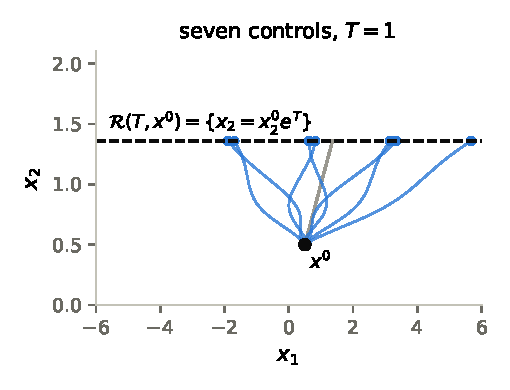
\includegraphics[width=\textwidth]{example_uncontrollable.pdf}

% \scriptsize Seven trajectories with different controls, $T=1$; the grey one has $u=0$. All end on the same line.
\end{column}
\end{columns}
\nbref{02 \S2}
\end{frame}


% =========================================================================
\begin{frame}{Example 2: the harmonic oscillator is controllable}
\begin{columns}[T]
\begin{column}{0.54\textwidth}
\footnotesize
With $A=\begin{pmatrix}0&1\\-1&0\end{pmatrix}$ and $B=\begin{pmatrix}0\\1\end{pmatrix}$ the system reads
\[
\begin{cases}
x_1'=x_2,\\
x_2'=-x_1+u
\end{cases}
\ \ \Longleftrightarrow\ \ x_1''+x_1=u .
\]


\medskip
To stop the oscillator, from $x^0=(1,0)$ to $x^1=(0,0)$, we can use a cubic polynomial
\[
u(t)=1-\frac{6}{T^2}+\frac{12\,t}{T^3}-3\Big(\frac tT\Big)^2+2\Big(\frac tT\Big)^3,
\]
with $\|u\|_{L^2(0,T)}=1.21$ for $T=5$.

\end{column}
\begin{column}{0.46\textwidth}
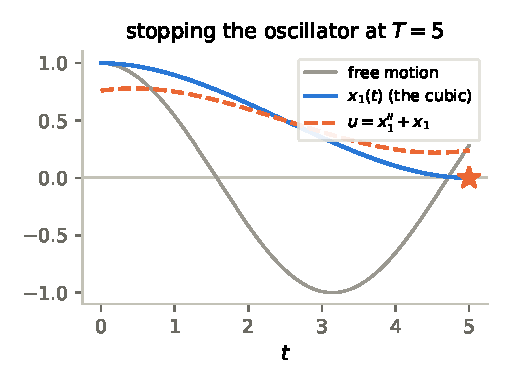
\includegraphics[width=\textwidth]{example_curve.pdf}

% \scriptsize The cubic and the free motion.
\end{column}
\end{columns}


\end{frame}


% =========================================================================
\begin{frame}{The reachable set}
\small
\begin{mathbox}{Definition (reachable set)}
The states that can be reached from $x^0$ in time $T$ form
\[
\Reach(T,x^0)=\big\{x(T)\;:\;x'=Ax+Bu,\ x(0)=x^0,\ u\in L^2(0,T;\R^m)\big\}.
\]
Controllability in time $T$ means $\Reach(T,x^0)=\R^n$ for every $x^0$.
\end{mathbox}
By variation of constants, $x(T)=e^{AT}x^0+L_Tu$ with the \alert{input-to-state map}
\[
L_T:L^2(0,T;\R^m)\to\R^n,\qquad L_Tu=\int_0^Te^{A(T-s)}Bu(s)\,ds ,
\]
which is linear, so $\Reach(T,x^0)=e^{AT}x^0+\Range L_T$ is an \alert{affine subspace}: the free evolution of $x^0$, plus everything the control can add.

\medskip
Which directions can the control add? Expand $e^{A(T-s)}B=\sum_{k\ge0}\frac{(T-s)^k}{k!}A^kB$: by \alert{Cayley--Hamilton}, $A^k\in\operatorname{span}\{I,A,\dots,A^{n-1}\}$ for $k\ge n$, so only the columns of $B,AB,\dots,A^{n-1}B$ ever appear.
\end{frame}


% =========================================================================
\begin{frame}{The Kalman rank condition}
\begin{mathbox}{Definition (Kalman matrix)}
\[
\Kal(A,B)=[\,B,\;AB,\;A^2B,\;\dots,\;A^{n-1}B\,]\in\R^{n\times nm}.
\]
\end{mathbox}
\begin{mathbox}{Theorem 1 (Kalman, 1960)}
The system $x'=Ax+Bu$ is controllable if and only if
\[
\rank\Kal(A,B)=n .
\]
\end{mathbox}
\footnotesize
\begin{itemize}
\item A \alert{finite computation}: $n-1$ matrix products and one rank. No differential equation needs to be solved.
\item \alert{Time plays no role}: controllable in a second if controllable in an hour, at the price of a larger control.
\end{itemize}

\smallskip
\alert{Example 1.} $B=e_1$, $AB=e_1$: $\Kal=\big(\begin{smallmatrix}1&1\\0&0\end{smallmatrix}\big)$ has rank $1$: not controllable, as found by hand.\\
\alert{Example 2.} $B=e_2$, $AB=e_1$: $\Kal=\big(\begin{smallmatrix}0&1\\1&0\end{smallmatrix}\big)$ has rank $2$: controllable, in every time.
\end{frame}


% =========================================================================
% \begin{frame}{The reachable set: two pictures}
% \begin{center}
% 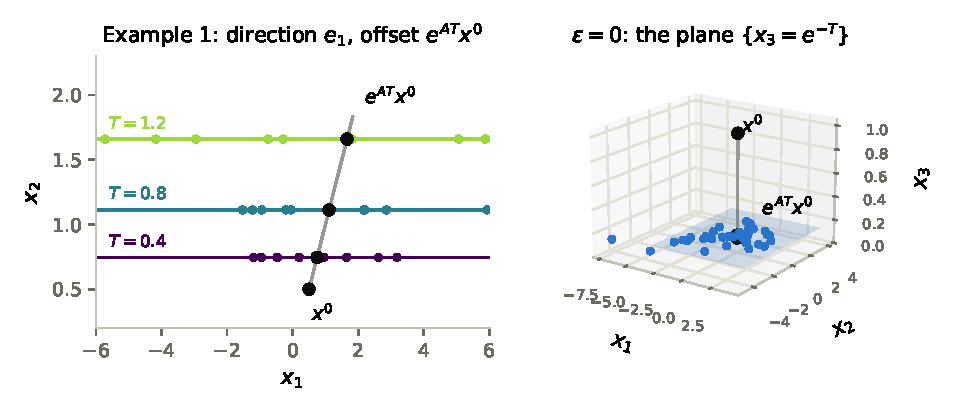
\includegraphics[width=0.76\textwidth]{reachable_set.pdf}
% \end{center}
% \footnotesize
% \alert{Left: Example 1} for three horizons. The reachable sets are parallel lines with direction $e_1$; their offset $e^{AT}x^0$ (black dots) moves along the free trajectory (grey). The coloured dots are the endpoints of trajectories with random controls.

% \medskip
% \alert{Right: three dimensions.} An oscillator $(x_1,x_2)$ coupled to a decaying mode $x_3'=-x_3$ that the control does not touch:
% $A=\begin{pmatrix}0&1&0\\-1&0&0\\0&0&-1\end{pmatrix}$, $B=\begin{pmatrix}0\\1\\0\end{pmatrix}$, $\Range\Kal=\{x_3=0\}$. From $x^0=(0,0,1)$ every reachable state at time $T$ lies on the plane $\{x_3=e^{-T}\}$, whatever the control. We will meet this family again.
% \nbref{02 \S4, Ex.~3}
% \end{frame}


% =========================================================================
\begin{frame}{Proof of Theorem 1}
\footnotesize
\alert{Necessity.} Since $\Reach(T,x^0)=e^{AT}x^0+\Range L_T$, controllability in time $T$ means $\Range L_T=\R^n$. The Cayley--Hamilton expansion of $e^{A(T-s)}B$ on the reachable-set slide shows that every $L_Tu$ is a combination of columns of $B,AB,\dots,A^{n-1}B$, so $\Range L_T\subseteq\Range\Kal$. Hence controllability forces $\rank\Kal=n$.

\smallskip
\alert{Sufficiency.} Assume $\rank\Kal=n$. Both ranges are subspaces of $\R^n$, so it suffices to show that every $v$ orthogonal to $\Range L_T$ is orthogonal to $\Range\Kal$. Let $v\perp\Range L_T$. For every control,
\[
0=\langle v,L_Tu\rangle=\int_0^T\big\langle B^*e^{A^*(T-s)}v,\,u(s)\big\rangle\,ds .
\]
\alert{Choose the control well.} Take $u(s)=B^*e^{A^*(T-s)}v$. Then $\int_0^T|B^*e^{A^*(T-s)}v|^2\,ds=0$. The integrand is continuous, so $g(s):=B^*e^{A^*(T-s)}v$ vanishes for all $s\in[0,T]$.

\alert{All derivatives vanish.} The function $g$ is smooth and vanishes identically, so all its derivatives vanish. At $s=T$,
\[
g^{(j)}(T)=(-1)^jB^*(A^*)^jv=0\qquad\text{for all }j\ge0 .
\]
In other words, $v$ is orthogonal to every column of $A^jB$, hence to $\Range\Kal=\R^n$. So $v=0$, and $\Range L_T=\R^n$: the system is controllable. \hfill$\square$

% \medskip
% \emph{Remark.} The control $u(s)=B^*e^{A^*(T-s)}v$ will reappear twice: in the Gramian below, and in the next lecture as the observation of an \emph{adjoint} system running backward from $t=T$.
\nbref{02 \S3}
\end{frame}


% =========================================================================
\begin{frame}[fragile]{Computing the rank}
\begin{columns}[T]
\begin{column}{0.48\textwidth}
\begin{lstlisting}
def kalman(A, B):   # [B | AB | ... | A^{n-1}B]
    cols = [B]
    for _ in range(A.shape[0] - 1):
        cols.append(A @ cols[-1])
    return torch.cat(cols, dim=1)

def num_rank(M):
    s = torch.linalg.svdvals(M)
    tol = max(M.shape) * eps * s[0]
    return int((s > tol).sum()), s
\end{lstlisting}
\end{column}
\begin{column}{0.52\textwidth}
\footnotesize
\alert{The near-uncontrollable family.}
\[
A=\begin{pmatrix}0&1&0\\-1&0&0\\0&0&-1\end{pmatrix},\qquad B_\varepsilon=\begin{pmatrix}0\\1\\\varepsilon\end{pmatrix}:
\]
For $\varepsilon=0$ the actuator acts only on the oscillator and $\Range\Kal=\{x_3=0\}$.
\end{column}
\end{columns}
\vspace{-3mm}
\footnotesize
Numerical rank of $[B]$, $[B,AB]$, $[B,AB,A^2B]$, and the singular values of $\Kal$:
\begin{center}
\renewcommand{\arraystretch}{1.0}
\begin{tabular}{@{}c ccc l@{}}
\toprule
$\varepsilon$ & $[B]$ & $[B,AB]$ & $[B,AB,A^2B]$ & singular values of $\Kal$ \\
\midrule
$0$   & 1 & 2 & 2 & 1.414, 1.000, 0.000 \\
$0.1$ & 1 & 2 & 3 & 1.414, 1.005, 0.141 \\
$0.3$ & 1 & 2 & 3 & 1.414, 1.052, 0.403 \\
\bottomrule
\end{tabular}
\end{center}
For $\varepsilon=0.1$ the pair is controllable, but it is \emph{nearly} uncontrollable.
\nbref{02 \S4}
\end{frame}


% =========================================================================

% =========================================================================


% =========================================================================
\begin{frame}{Combining motions: parking}
\begin{center}
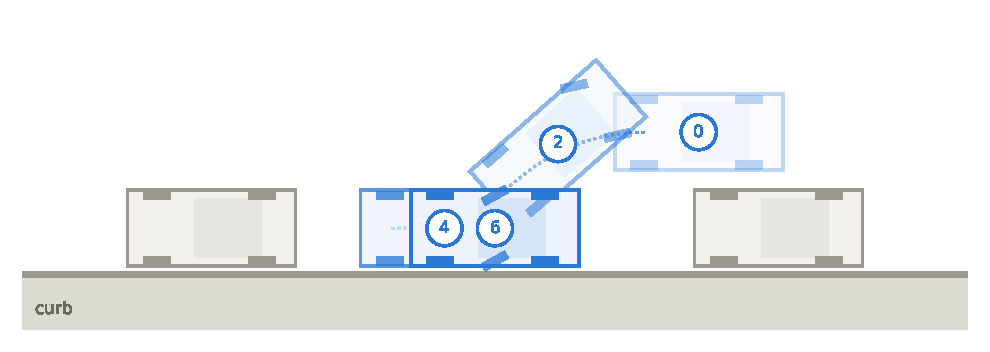
\includegraphics[width=0.84\textwidth]{parking.pdf}
\end{center}
\footnotesize
A car has two controls, \alert{drive} and \alert{steer}, but a four-dimensional state: position, heading and the angle of the wheels. No control moves it \emph{sideways}, which is what parallel parking requires. Six moves do it:
\begin{center}
\begin{tabular}{@{}cl cl cl@{}}
1 & steer right & 2 & reverse (the rear swings in) & 3 & steer left \\
4 & reverse (the nose swings in) & 5 & straighten the wheels & 6 & pull forward \\
\end{tabular}
\end{center}
New directions are generated by \emph{combining} motions that are available. This is the mechanism behind the Kalman matrix.
\end{frame}


\begin{frame}{Nelson's car and Lie brackets}
\footnotesize
State $(x,y,\theta,\varphi)$: position of the rear axle, heading, wheel angle. Controls: speed $v$ and steering rate $\omega$ (Nelson's car \citep{nelson1967}):
\[
\begin{pmatrix}x\\y\\\theta\\\varphi\end{pmatrix}'
= v\underbrace{\begin{pmatrix}\cos\theta\\ \sin\theta\\ \tfrac1L\tan\varphi\\ 0\end{pmatrix}}_{g_1:\ \text{drive}}
+\omega\underbrace{\begin{pmatrix}0\\0\\0\\1\end{pmatrix}}_{g_2:\ \text{steer}} .
\]
%At every state only the two directions $g_1,g_2$ are available, in a four-dimensional space. 
Going along $g_2$, then $g_1$, then back along $g_2$, then back along $g_1$ does \emph{not} return to the start: the net displacement is the \alert{Lie bracket}
\[
[g_2,g_1]=Dg_1\,g_2-Dg_2\,g_1=\Big(0,\,0,\,\tfrac{1}{L\cos^2\varphi},\,0\Big):\ \text{\emph{wriggle}},
\]
and $[[g_2,g_1],g_1]$ at $\varphi=0$ is $\tfrac1L(-\sin\theta,\cos\theta,0,0)$: \emph{slide}, sideways. Drive, steer, wriggle and slide span $\R^4$: the car is controllable \citep{sontag1998,coron2007}.

\begin{mathbox}{The linear case}
For $x'=Ax+bu$ the drift is $f(x)=Ax$ and the control field is the constant $b$: $[f,b]=Db\,f-Df\,b=-Ab$. Brackets with the drift produce $Ab,A^2b,\dots$: the Kalman matrix is the linear instance of a rank condition on Lie brackets.
\end{mathbox}
\nbref{02 \S8}
\end{frame}



\begin{frame}{The Kalmann rank, block by block}
\begin{columns}[T]
\begin{column}{0.56\textwidth}
Consider the dynamical system
$$ x^{(n)}=u $$
which is the simplest controllable system.
\medskip
\alert{Every block is needed:} For the state $(x,x',\dots,x^{(n-1)})$,
\[
A=\begin{pmatrix}0&1&&\\&0&\ddots&\\&&\ddots&1\\&&&0\end{pmatrix},\qquad B=e_n,
\]
so $B=e_n,\ AB=e_{n-1},\ \dots,\ A^{n-1}B=e_1$.
\end{column}
\begin{column}{0.44\textwidth}
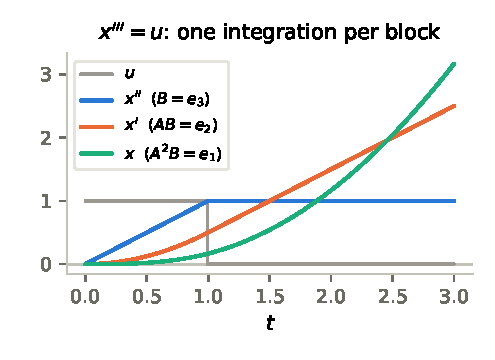
\includegraphics[width=\textwidth]{integrator_chain.pdf}

\scriptsize $x'''=u$ with $u$ a unit pulse on $[0,1]$: the pulse enters $x''$ at once, $x'$ after one integration and $x$ after two. Each block of the Kalman matrix is one integration.
\end{column}
\end{columns}
\nbref{02 \S5, Ex.~4}
\end{frame}





\begin{frame}{Most systems are controllable}
\footnotesize
\alert{Controllable pairs are open and dense.} Controllability fails if and only if all $n\times n$ minors of $\Kal(A,B)$ vanish. Each minor is a polynomial in the entries of $(A,B)$. The set where finitely many polynomials vanish, not all of them identically zero, is closed and has empty interior. So controllability is
\begin{itemize}
\item \alert{robust}: it survives small perturbations of $A$ and $B$;
\item \alert{generic}: most systems are controllable, and an arbitrarily small perturbation makes an uncontrollable pair controllable.
\end{itemize}

\medskip
\alert{Rank is not a measure of ``how controllable''.} A pair can be controllable \emph{and} nearly uncontrollable, like the family at $\varepsilon=0.1$. The singular values tell more than the rank.

\medskip
\alert{Cost estimate.} When controllability holds there is a control with
\[
\|u\|_{L^2(0,T)}\le C\,\big|e^{AT}x^0-x^1\big|,
\]
where $C$ depends on $(A,B,T)$. The size of $C$ is the quantitative side of controllability. The Gramian, below, makes it computable.
\end{frame}



% =========================================================================


% =========================================================================
\section{The Gramian and the cost of control}

\begin{frame}{The controllability Gramian}
\small
The proof of Theorem 1 used the control $u(s)=B^*e^{A^*(T-s)}v$. Applying $L_T$ to controls of this form produces a matrix.
\begin{mathbox}{Definition (controllability Gramian)}
\[
\Gram_T=\int_0^Te^{A(T-s)}BB^*e^{A^*(T-s)}\,ds\in\R^{n\times n}.
\]
\end{mathbox}
\begin{mathbox}{Proposition 2 (properties of the Gramian)}
\begin{enumerate}
\item $\Gram_T$ is symmetric and positive semidefinite: $v^*\Gram_Tv=\int_0^T|B^*e^{A^*(T-s)}v|^2ds\ge0$.
\item $\ker\Gram_T=(\Range\Kal)^\perp$.
\item $\Gram_T$ is invertible if and only if $\rank\Kal=n$, that is, if and only if the system is controllable.
\item $L_T\big(B^*e^{A^*(T-\cdot)}c\big)=\Gram_Tc$ for every $c\in\R^n$.
\end{enumerate}
\end{mathbox}
One $n\times n$ matrix records how strongly the control acts in each direction of the state space over $[0,T]$.
\end{frame}


% =========================================================================
\begin{frame}{Proof of Proposition 2}
\small
\alert{(1)} Symmetry is clear from the formula, since $\big(e^{A\tau}BB^*e^{A^*\tau}\big)^*$ is the same matrix. The identity follows from $v^*e^{A(T-s)}BB^*e^{A^*(T-s)}v=|B^*e^{A^*(T-s)}v|^2$, integrated over $s$.

\medskip
\alert{(2)} If $\Gram_Tv=0$ then $v^*\Gram_Tv=0$, hence $g(s)=B^*e^{A^*(T-s)}v\equiv0$ by (1), and the derivative argument in the proof of Theorem 1 gives $v\perp\Range\Kal$.

Conversely, if $v\perp\Range\Kal$, then $v$ is orthogonal to every column of $e^{A(T-s)}B$ by the Cayley--Hamilton step in the proof of Theorem 1. So $g\equiv0$, and $\Gram_Tv=\int_0^Te^{A(T-s)}B\,g(s)\,ds=0$.

\medskip
\alert{(3)} By (2), $\Gram_T$ is invertible iff $(\Range\Kal)^\perp=\{0\}$ iff $\Range\Kal=\R^n$ iff $\rank\Kal=n$, which is controllability by Theorem 1.

\medskip
\alert{(4)} By the definition of $L_T$ applied to $u(s)=B^*e^{A^*(T-s)}c$,
\[
L_Tu=\int_0^Te^{A(T-s)}B\,B^*e^{A^*(T-s)}c\,ds=\Gram_Tc . \qquad\square
\]
\end{frame}


% =========================================================================
\begin{frame}{An explicit steering control}
\small
If the system is controllable, property (4) tells us how to reach any target. We want $L_Tu=x^1-e^{AT}x^0$; try $u=B^*e^{A^*(T-\cdot)}c$ and solve $\Gram_Tc=x^1-e^{AT}x^0$:
\begin{mathbox}{The Gramian control}
\[
u(t)=B^*e^{A^*(T-t)}\,\Gram_T^{-1}\big(x^1-e^{AT}x^0\big).\tag{G}
\]
\end{mathbox}
\alert{Verification.} By variation of constants and the definition of $\Gram_T$,
\[
\begin{aligned}
x(T)&=e^{AT}x^0+\int_0^Te^{A(T-s)}BB^*e^{A^*(T-s)}\,ds\;\Gram_T^{-1}\big(x^1-e^{AT}x^0\big)\\
&=e^{AT}x^0+\Gram_T\,\Gram_T^{-1}\big(x^1-e^{AT}x^0\big)=x^1 .
\end{aligned}\qquad\square
\]
% \alert{What we have.} A formula that steers \emph{any} $x^0$ to \emph{any} $x^1$ in \emph{any} time $T$, for \emph{every} controllable pair $(A,B)$: one integral and one $n\times n$ linear solve. Compare with Example 2, where a curve had to be guessed for one particular equation.

\medskip
\alert{What we do not have yet.} Why this particular form $u=B^*e^{A^*(T-\cdot)}c$? Is it the cheapest control? The next lecture answers both: it is the control of \emph{minimal $L^2$ norm}, and it comes from a dual, \emph{adjoint} problem.
\end{frame}


% =========================================================================
\begin{frame}{The control (G) stops the oscillator}
\begin{center}
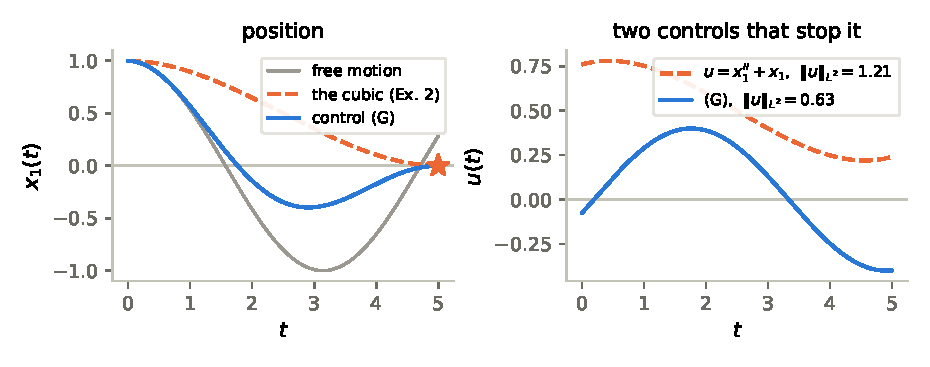
\includegraphics[width=0.84\textwidth]{gramian_control.pdf}
\end{center}
\small
For $A=\begin{pmatrix}0&1\\-1&0\end{pmatrix}$, $B=e_2$ and $T=5$: $\Kal=[B,AB]=\begin{pmatrix}0&1\\1&0\end{pmatrix}$ has rank $2$, and
\[
\Gram_T=\begin{pmatrix}2.636&0.460\\0.460&2.364\end{pmatrix},\qquad \lambda(\Gram_T)=\{2.02,\ 2.98\}.
\]
% Both controls stop the oscillator, $|x(T)-x^1|<10^{-5}$, and (G) does it with half the effort of the cubic. The cubic was one guess among infinitely many; (G) is singled out by the structure of the problem.
% \nbref{02 \S6}
\end{frame}


% =========================================================================
\begin{frame}{The cost of control}
\alert{The effort of (G).} With $d=x^1-e^{AT}x^0$ and $c=\Gram_T^{-1}d$,
\[
\int_0^T|u(t)|^2dt=\int_0^Tc^*e^{A(T-t)}BB^*e^{A^*(T-t)}c\,dt=c^*\Gram_Tc=d^*\Gram_T^{-1}d .
\]
And the constant in the cost estimate is $\lambda_{\min}(\Gram_T)^{-1/2}$: the smallest eigenvalue of the Gramian measures the hardest direction.

\medskip
\alert{Longer horizons are cheaper.} %With $\tau=T-s$, $\Gram_T=\int_0^Te^{A\tau}BB^*e^{A^*\tau}\,d\tau$,
For $T'>T$
\[
\Gram_{T'}-\Gram_T=\int_T^{T'}e^{A\tau}BB^*e^{A^*\tau}\,d\tau\succeq0 .
\]
Thus $\lambda_{\min}(\Gram_T)$ is non-decreasing in $T$, and the same displacement $d$ costs no more effort on a longer horizon.

% \medskip
% \alert{Direction by direction.} In the eigenbasis of $\Gram_T$, $d^*\Gram_T^{-1}d=\sum_i d_i^2/\lambda_i$: a target component along an eigenvector with small $\lambda_i$ is expensive. The rank says \emph{whether}; the Gramian says \emph{how much}.
% \nbref{02 Ex.~5}
\end{frame}


% =========================================================================
\begin{frame}{How hard is it to control? The near-uncontrollable family}
\begin{columns}[T]
\begin{column}{0.58\textwidth}
\footnotesize
The Kalman condition is a yes/no answer, and a ``yes'' can hide very different behaviours. Take again
\[
A=\begin{pmatrix}0&1&0\\-1&0&0\\0&0&-1\end{pmatrix},\qquad B_\varepsilon=\begin{pmatrix}0\\1\\\varepsilon\end{pmatrix}.
\]
A direct computation gives $\det\Kal(A,B_\varepsilon)=-2\varepsilon$: controllable for every $\varepsilon\ne0$.

\medskip
Steering $x^0=0$ to the weak mode $e_3$ in time $T=5$ with (G) costs
\[
\int_0^T|u|^2dt=d^*\Gram_T^{-1}d\;\sim\;\frac{C}{\varepsilon^{2}}\qquad(\varepsilon\to0),
\]
at $\varepsilon=10^{-3}$ it is $10^6$ times its value at $\varepsilon=1$. 
% The weak mode is reached only through the coupling, and the price is its inverse square. The rank is algebraic; the singular values of $\Kal$ and the eigenvalues of $\Gram_T$ measure \emph{how hard} control is.
\end{column}
\begin{column}{0.42\textwidth}
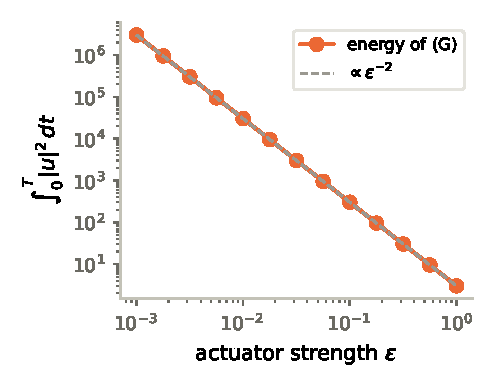
\includegraphics[width=\textwidth]{near_uncontrollable.pdf}

\scriptsize The energy of the control (G) against the coupling $\varepsilon$, on logarithmic axes.
\end{column}
\end{columns}
\nbref{02 \S7}
\end{frame}


% =========================================================================
% =========================================================================
\section{Outlook}

\begin{frame}{Control $\leftrightarrow$ machine learning}
\footnotesize
\begin{itemize}
\item \alert{Feedback $\leftrightarrow$ reinforcement learning.} Reinforcement learning is ``learning based on feedback'': there are no correct input--output pairs, but there is a reward. In both, an action depends on the observed state. A feedback law is \emph{designed} from a known model; a policy is \emph{learned} from rewards.
\item \alert{Damping $\leftrightarrow$ momentum.} The heavy-ball picture of momentum in gradient descent is a damped second-order dynamics. Its damping parameter can be too small, giving oscillations, or too large, giving slow creeping, as in the overdamping paradox of Part I.
% \item \alert{One system $\leftrightarrow$ many trajectories.} Classical controllability asks whether \emph{one} system can be steered by \emph{its} control. Supervised learning with a neural ODE, $x'=w(t)\,\sigma\big(a(t)\cdot x+b(t)\big)$, is \emph{simultaneous} control: \emph{many} trajectories, one per data point, steered by \emph{one shared} control, the parameters. The rank argument does not apply there; geometric constructions will.
% \item \alert{Discrete time.} A residual layer $x_{k+1}=x_k+h\,w_k\,\sigma(a_k\cdot x_k+b_k)$ is one Euler step of that system, and training is an optimal control problem over the layers.
\end{itemize}
\end{frame}


% =========================================================================
\begin{frame}{The overdamping paradox}
\begin{columns}[T]
\begin{column}{0.53\textwidth}
\footnotesize
\alert{The model.} Without friction, the linearized pendulum $x_1''+x_1=0$ conserves its energy
\[
e(t)=\tfrac12\big(x_1(t)^2+x_1'(t)^2\big).
\]
With friction proportional to the velocity,
\[
x_1''+x_1=-k\,x_1',\qquad k>0 .
\]
The control is $u=-kx_2$: a feedback law where the control opposes the measured velocity. It is the simplest instance of Maxwell's governor analysis.

\medskip
\alert{Energy decreases.} Along solutions,
\[
e'(t)=x_1'\,(x_1+x_1'')=-k\,(x_1')^2\;\le\;0 .
\]
So more damping removes energy faster \emph{at each instant}, for the same velocity.

\medskip
\alert{Does it follow that a larger $k$ always brings the system to rest faster?}
\end{column}
\begin{column}{0.45\textwidth}
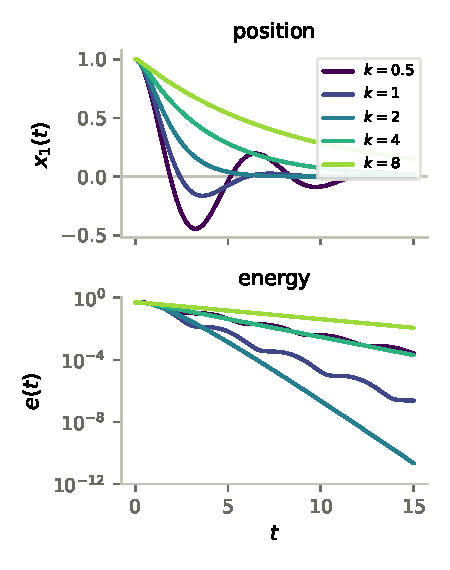
\includegraphics[width=\textwidth]{overdamping.pdf}
\end{column}
\end{columns}
\nbref{01 \S4}
\end{frame}


% =========================================================================
\begin{frame}{Beyond linear, finite-dimensional, unconstrained}
\footnotesize
\begin{itemize}
\item \alert{Nonlinear systems.} If the linearization at an equilibrium is controllable, the nonlinear system is controllable \emph{near} it. Far from equilibria, Lie brackets replace the Kalman blocks (parking). Controllability can be global, local, or fail altogether.
\item \alert{Bounded controls.} With $|u(t)|\le1$ the reachable set is no longer a subspace but a convex set that grows with $T$; time-optimal controls switch between the extreme values: \emph{bang-bang}.
% \item \alert{The heat equation.} $y_t=\Delta y+\mathbf 1_\omega u$ is \emph{approximately} controllable in any time $T>0$ from any subregion $\omega$, but not exactly: the solution is smooth at time $T$ whatever the control, so rough targets are out of reach. Smoothing is an obstruction.
% \item \alert{The wave equation.} Exact controllability holds if and only if $T$ is large enough for the waves to travel from $\omega$ to the whole domain, and $\omega$ satisfies a geometric condition: every ray must meet it \citep{zuazua2007}. Finite propagation speed is an obstruction.
\item \alert{Stochastic systems.} Controls act on distributions; the natural questions are about expectations and risks, and feedback becomes indispensable.
\end{itemize}
\end{frame}


% =========================================================================
\begin{frame}{Observation: we rarely see the whole state}
\small
In practice we only \alert{observe an output}
\[
x'(t)=f\big(x(t),u(t)\big),\qquad \alert{y(t)=g\big(x(t)\big)}\in\R^p,\qquad\text{usually } p<n .
\]
In the linear case, $x'=Ax+Bu$ and $y=Cx$ with $C\in\R^{p\times n}$.

\medskip
\footnotesize
\renewcommand{\arraystretch}{1.25}
\begin{tabularx}{\textwidth}{@{}>{\raggedright\arraybackslash}p{0.27\textwidth} >{\raggedright\arraybackslash}p{0.33\textwidth} >{\raggedright\arraybackslash}X@{}}
\toprule
\textbf{System} & \textbf{State $x$} & \textbf{Observation $y$} \\
\midrule
oscillator, pendulum & position and velocity & position only: $C=(1\;\;0)$ \\
heat in a domain $\Omega$ & temperature field & thermometers in a subregion $\omega\subset\Omega$ \\
a spacecraft & position, velocity, attitude & radar ranges, star sightings \\
reinforcement learning & the state of the environment & a camera image of it \\
\bottomrule
\end{tabularx}

\bigskip
\begin{center}
\normalsize\alert{Knowing $u$ and $y$ on $(0,T)$, can we recover $x(t)$? Can we still stabilize?}
\end{center}
\end{frame}


% =========================================================================
% \begin{frame}{Observability}
% \small
% \alert{The question.} The control is known, so by linearity we may take $u=0$. Then $y(t)=Ce^{At}x^0$ for $t\in(0,T)$, and the pair $(A,C)$ is \alert{observable} if $y\equiv0$ on $(0,T)$ forces $x^0=0$: the observation determines the initial state, hence the whole trajectory.

% \medskip
% \alert{The answer.} Since $y^{(k)}(0)=CA^kx^0$, the argument of Theorem~1 gives
% \[
% (A,C)\ \text{observable}\iff\rank\begin{pmatrix}C\\ CA\\ \vdots\\ CA^{n-1}\end{pmatrix}=n\iff(A^*,C^*)\ \text{controllable},
% \]
% because the transpose of this matrix is $\Kal(A^*,C^*)$. Observing and controlling are \alert{dual} problems.

% \smallskip
% \footnotesize
% \begin{itemize}
% \item Oscillator ($k=m_0=1$), position measured: $C=(1\;\;0)$, $CA=(0\;\;1)$, rank $2$. The velocity can be read off the positions.
% \item Free particle $q''=u$, velocity measured: $A=\begin{psmallmatrix}0&1\\0&0\end{psmallmatrix}$, $C=(0\;\;1)$, $CA=(0\;\;0)$, rank $1$. A speedometer never tells where you are.
% \end{itemize}
% \end{frame}


% % =========================================================================
% \begin{frame}{What can we do? Estimate the state, then feed it back}
% \begin{center}
% \begin{tikzpicture}[>=Stealth, thick,
%   block/.style={draw=boxframe, fill=boxbg, rounded corners=2pt, align=center, font=\footnotesize, inner sep=4pt}]
%   \node[block] (plant) {system\\[1pt] $x'=Ax+Bu,\ \ y=Cx$};
%   \node[block, right=16mm of plant] (obs) {observer\\[1pt] $\hat x'=A\hat x+Bu+L(y-C\hat x)$};
%   \node[block] (gain) at ($(plant)!0.5!(obs)+(0,-1.3)$) {$u=-K\hat x$};
%   \draw[->] (plant) -- node[above, font=\footnotesize]{$y$} (obs);
%   \draw[->] (obs.south) |- node[pos=0.75, below, font=\footnotesize]{$\hat x$} (gain.east);
%   \draw[->] (gain.west) -| node[pos=0.25, below, font=\footnotesize]{$u$} (plant.south);
% \end{tikzpicture}
% \end{center}
% \footnotesize
% \alert{An observer} \citep{luenberger1964} is a copy of the model, corrected by the mismatch with the measurement. The error $e=x-\hat x$ solves $e'=(A-LC)\,e$.
% If $(A,C)$ is observable, the eigenvalues of $A-LC$ can be chosen freely (pole placement for the dual pair $(A^*,C^*)$, Notebook 05), so $\hat x(t)\to x(t)$ exponentially. As with damping, faster is not always better: a fast observer amplifies the measurement noise.

% \medskip
% \alert{Separation.} With $u=-K\hat x$, the closed loop has the eigenvalues of $A-BK$ and of $A-LC$: the feedback and the observer are designed independently. With noisy measurements, the best $L$ solves a Riccati equation: the \alert{Kalman filter} \citep{kalman1960filter}, which navigated Apollo \citep{hoag1969}.

% \medskip
% \alert{Next lecture.} The control (G) is itself an observation: $u(s)=B^*\varphi(s)$, where $\varphi'=-A^*\varphi$. Duality is how controls are built.
% \end{frame}


% =========================================================================
% \begin{frame}{Where are we going?}
% \footnotesize
% We know \emph{when} a linear system is controllable (Kalman), and we have an \emph{explicit} control (G). Why this control, whether it is the cheapest, and why $B^*e^{A^*(T-s)}v$ keeps appearing are the questions of the next lecture.

% \medskip
% \renewcommand{\arraystretch}{1.15}
% \begin{tabular}{@{}p{0.07\textwidth} p{0.40\textwidth} p{0.47\textwidth}@{}}
% \toprule
%  & \textbf{Notebook} & \textbf{Question} \\
% \midrule
% 01 & What is control? & states, controls, targets, feedback; the overdamping paradox \\
% 02 & Linear control and the Kalman condition & reachable sets, the Gramian, the control (G) \\
% 03 & Observability, duality and adjoints & why (G) is the cheapest control; adjoint systems \\
% 04 & Bang-bang and switching controls & bounded controls, time-optimal control \\
% 05 & Feedback stabilization, LQR and MPC & the rule $u=-Kx$; the Riccati equation \\
% 06--08 & Optimization, adjoints, turnpike & gradient flows, the heat equation, long horizons \\
% 09--19 & Machine learning as control & training, ResNets, transformers, diffusion, RL \\
% \bottomrule
% \end{tabular}

% \medskip
% Notebooks and slides: \url{https://cml-fau.github.io/}
% \end{frame}


% =========================================================================
\begin{frame}{Part II: key takeaways}
\footnotesize
\begin{enumerate}
% \item Variation of constants: $x(T)=e^{AT}x^0+L_Tu$ with $L_Tu=\int_0^Te^{A(T-s)}Bu(s)\,ds$.
% \item Reachable set: $\Reach(T,x^0)=e^{AT}x^0+\Range\Kal(A,B)$.
\item Kalman: controllable $\iff$ $\rank[B,AB,\dots,A^{n-1}B]=n$.
% \item The proof uses Cayley--Hamilton ($\subseteq$) and the vanishing of all derivatives of $B^*e^{A^*(T-s)}v$ at $s=T$ ($\supseteq$). The rank of $[B,AB,\dots,A^kB]$ grows until it stalls and then stays; the chain of integrators $x^{(n)}=u$ needs all $n$ blocks.
\item New directions come from combining motions: $AB$ for linear systems, Lie brackets for the car.
% \item Gramian: $\Gram_T$ is symmetric, positive semidefinite, with $\ker\Gram_T=(\Range\Kal)^\perp$; it is invertible iff the system is controllable.
\item The Gramian measures the effort needed to steer $x^0$ to $x^1$.
\item The rank is algebraic; singular values and Gramian eigenvalues measure how hard control is, direction by direction.
% \item Feedback can be too strong: the decay rate of $x''+kx'+x=0$ is maximal at $k=2$ and tends to $0$ as $k\to\infty$.
\end{enumerate}
\end{frame}


% =========================================================================
\begin{frame}[allowframebreaks]{References}
\scriptsize
\bibliographystyle{plainnat}
\bibliography{introduction_control_theory}
\end{frame}

\end{document}
